% !TeX root = d2.tex

\documentclass{article}

% \usepackage{xcolor}
\usepackage[margin=0.5in]{geometry} 
\usepackage{graphicx}
\usepackage{multirow}
\usepackage[table,xcdraw]{xcolor}
\usepackage[normalem]{ulem}
\usepackage{float}
\usepackage{adjustbox, lipsum}
\usepackage{pdfpages}
\useunder{\uline}{\ul}{}
\title{MindMerge --- Deliverable e 2}
\author{Gabriele Benetti, Gioele Bernardini, Luca Fossa Crescini, Luca Sartore}

\begin{document}
\maketitle


\tableofcontents


\newpage
\section*{Abstract}   % titolo temporaneo da modificare
This is the Abstract of the deliverable 2

\section{Architecture description}


\begin{figure}[h]
  \centering
  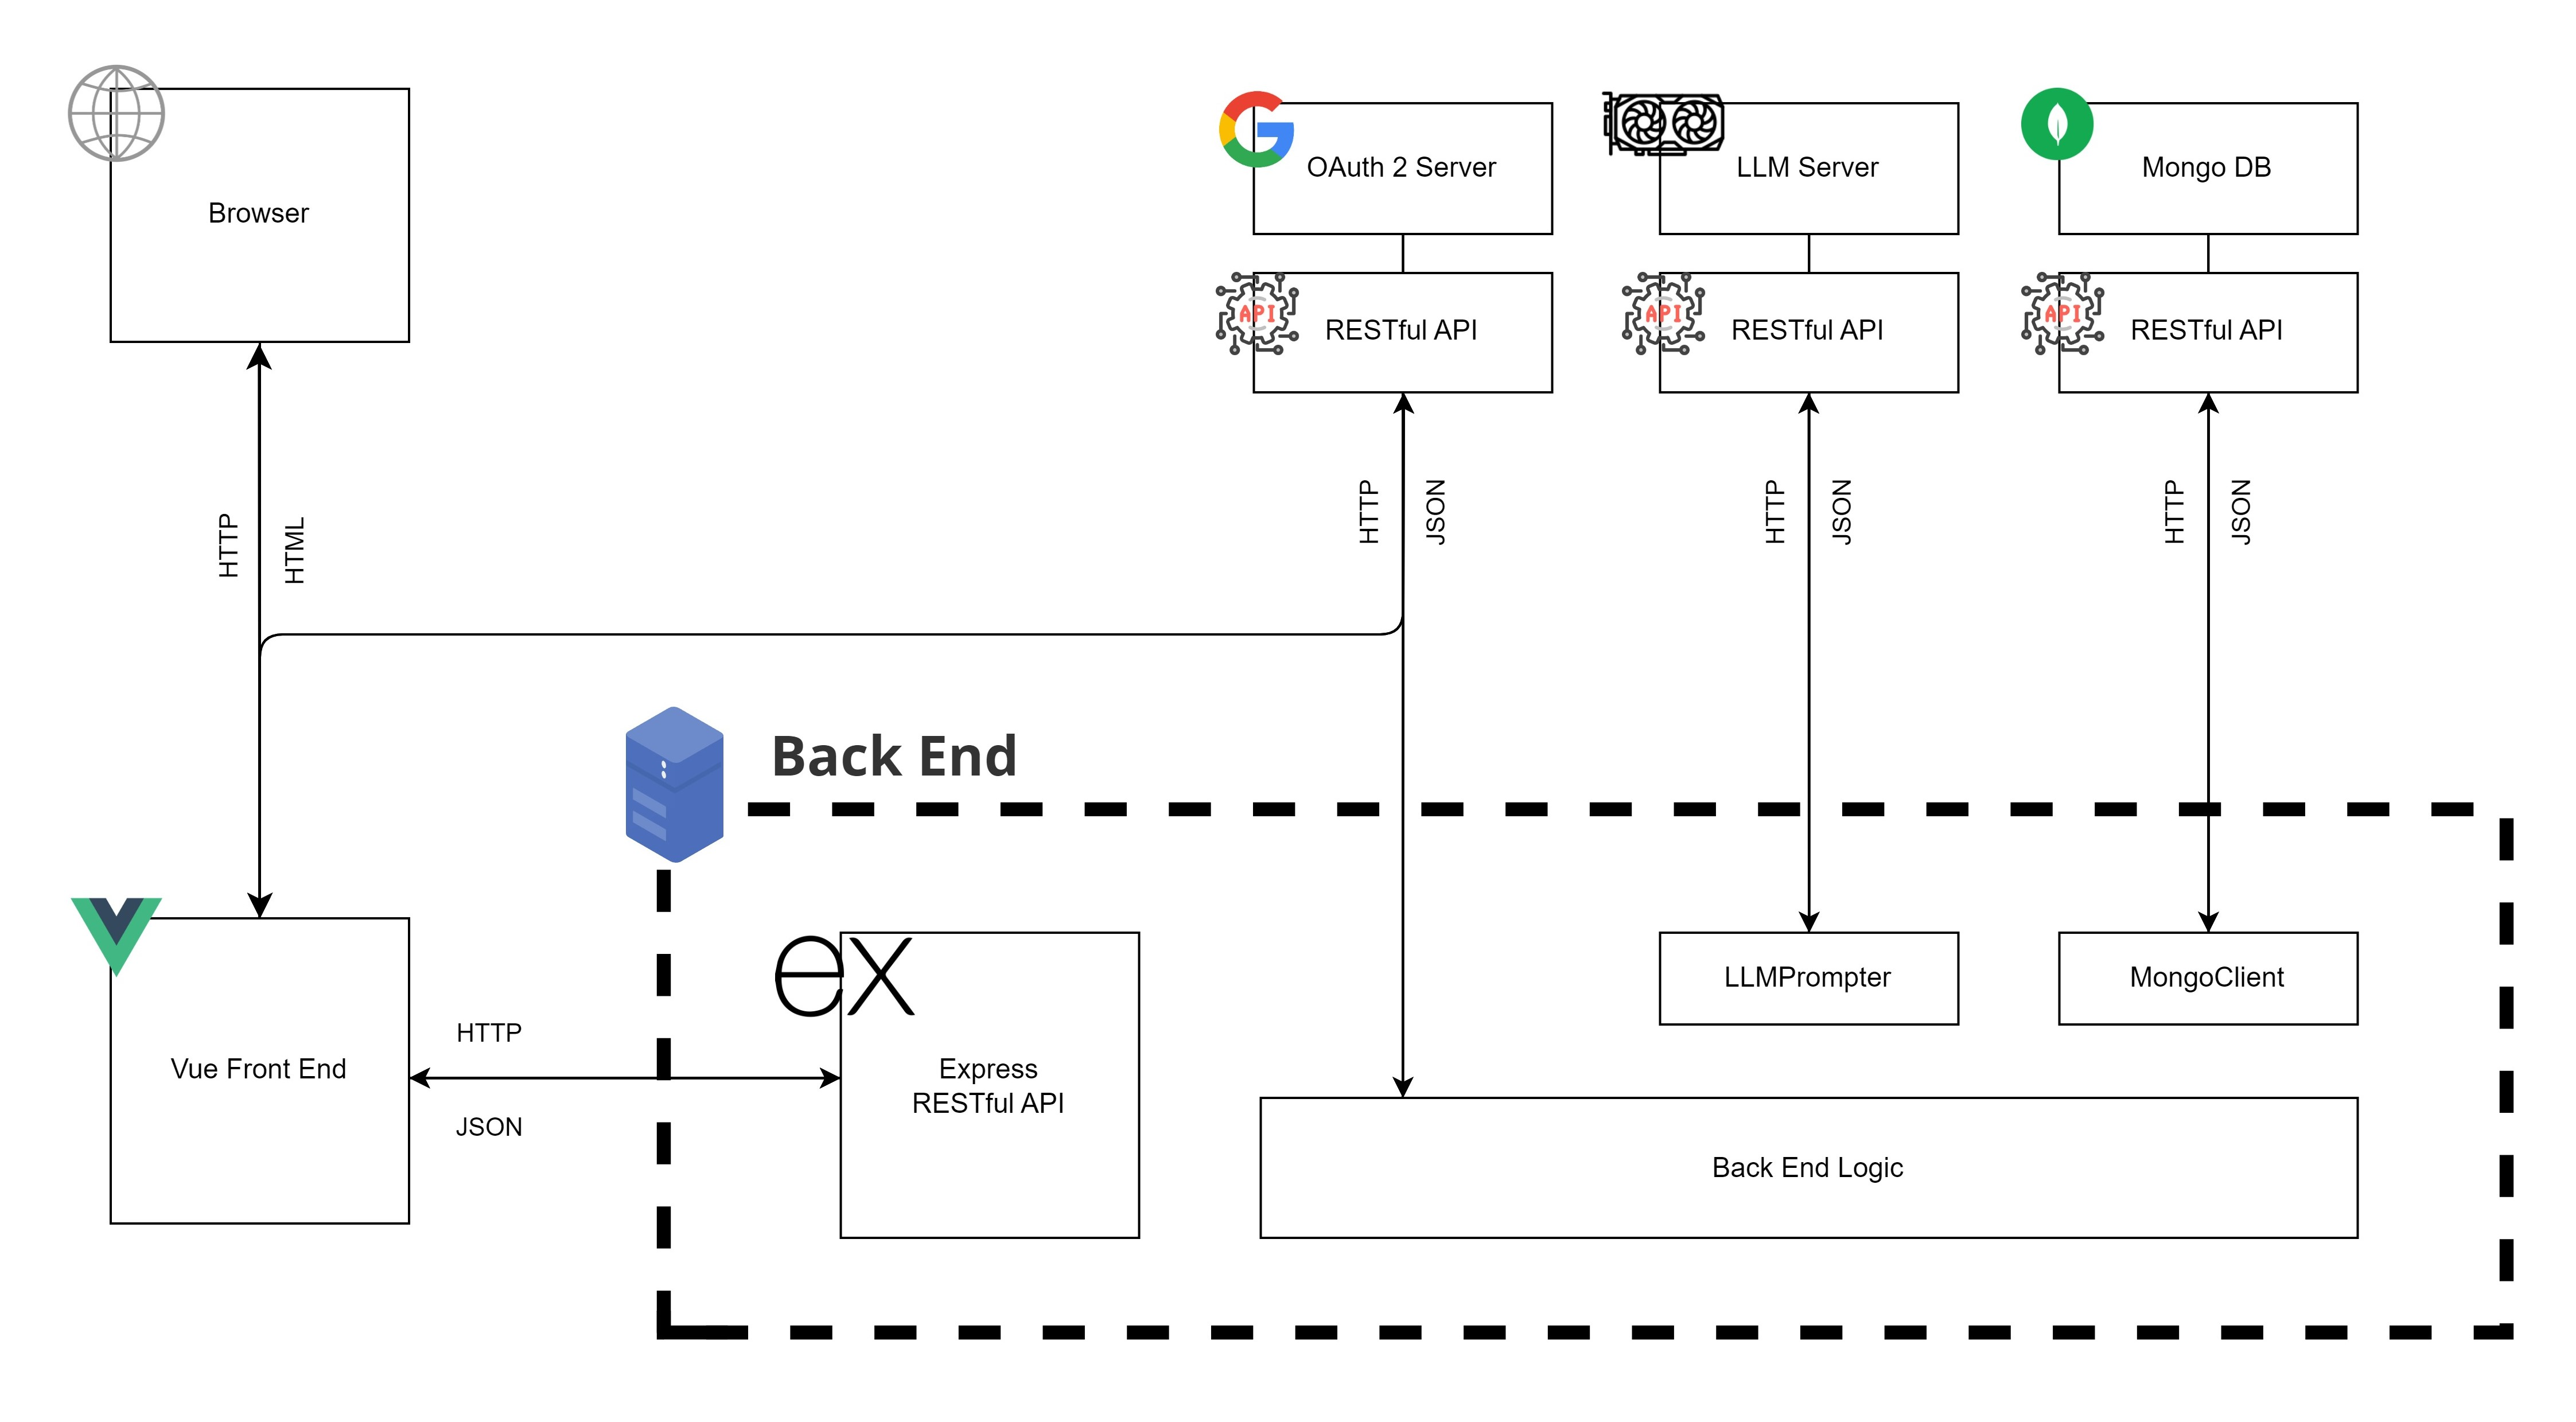
\includegraphics[width=0.95\textwidth]{images/architecture.jpg}
  \caption{\small The architecture diagram ot the MindMerge system}
\end{figure}
The architecture is relatively simple,
comprising two classical components: the front end and the back end, along with several smaller components (browser, OAuth server, LLM service, and MongoDB).
\newline \newline
The browser communicates with the front end using the HTTP protocol and HTML format.
\newline \newline
The front end, based on the Vue library, accesses resources provided by the back end using HTTP with JSON data format.
\newline \newline
Authentication is provided by a third-party OAuth server, that communicate with both the front end and back end via HTTP/JSON.
\newline \newline
The back end is the most complex component consists of several sub-components, including:
\begin{itemize}
  \item A part providing RESTful APIs based on Express.js
  \item A component dedicated to communicating with the database (MongoClient)
  \item A module for communicating with the LLM service (LLMPrompter)
  \item Logic containing all functions necessary for the application's operation.
\end{itemize}
All the communications that the backend has with the external world are made through HTTP with json format.

\section{Product Backlog}


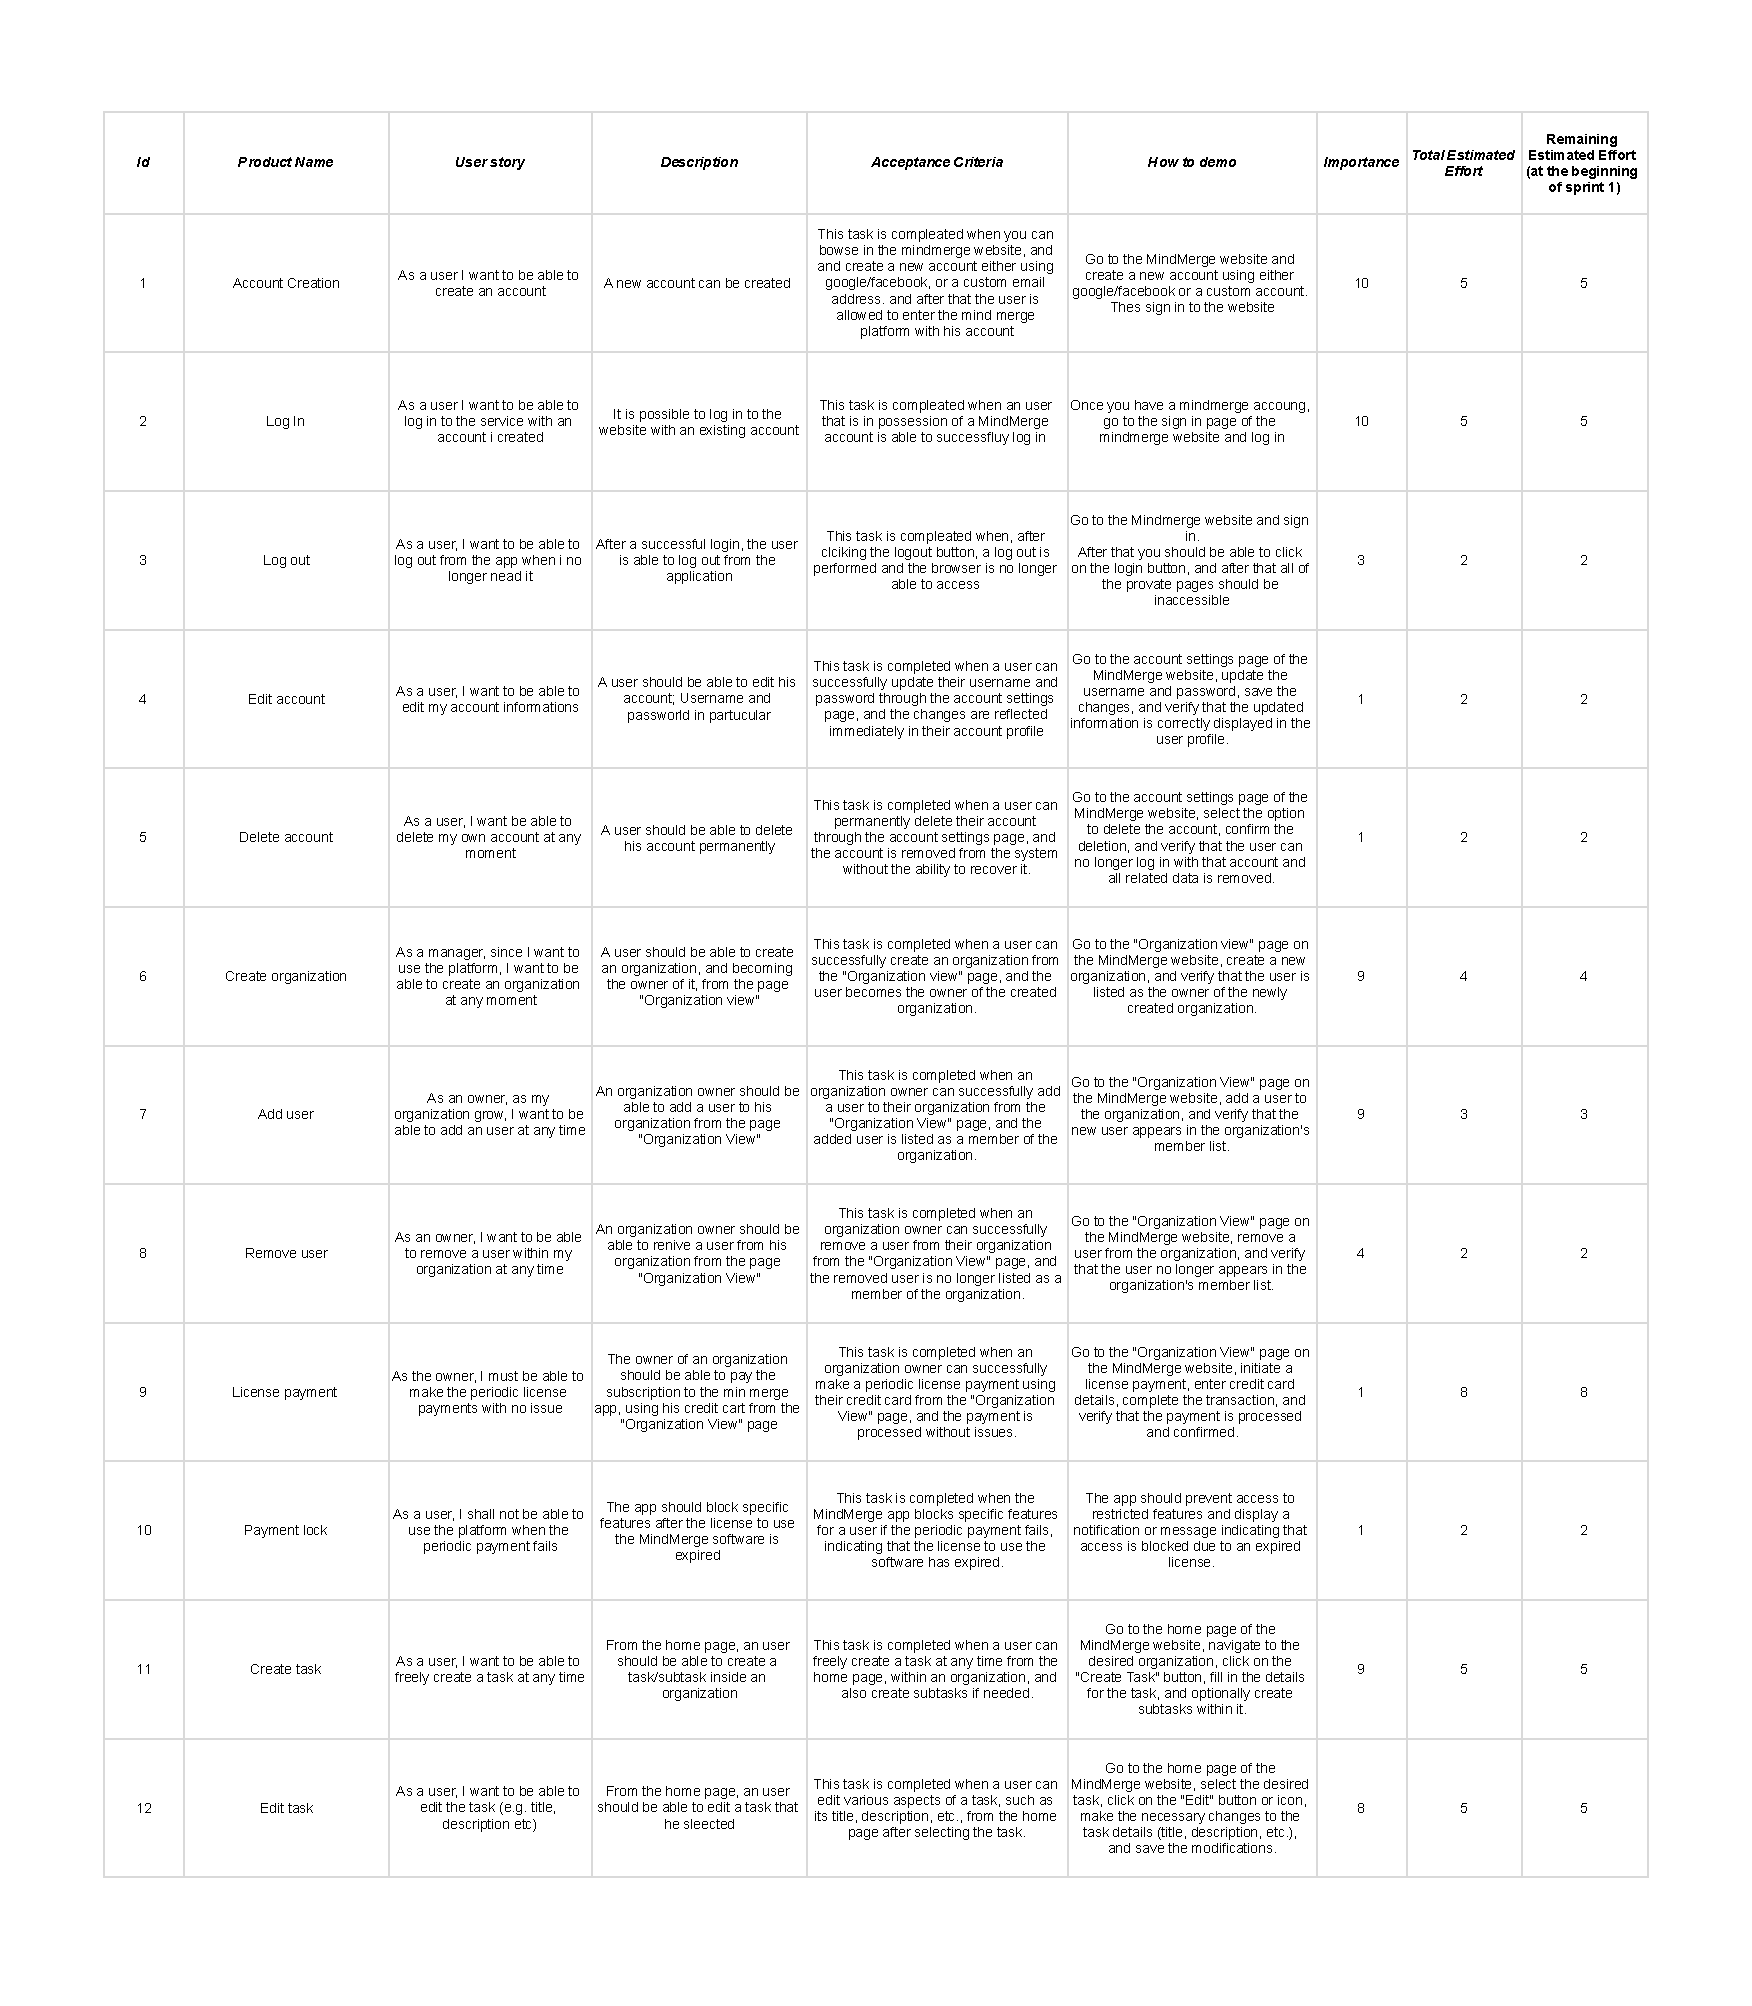
\includepdf[pages=-]{images/product_backlog.pdf}

\section{Definition of Tests}

\subsection*{Test DatabaseManager:TaskManager}
This section contains the tests for the TaskManager class, which is responsible for managing tasks in the database.
\newline
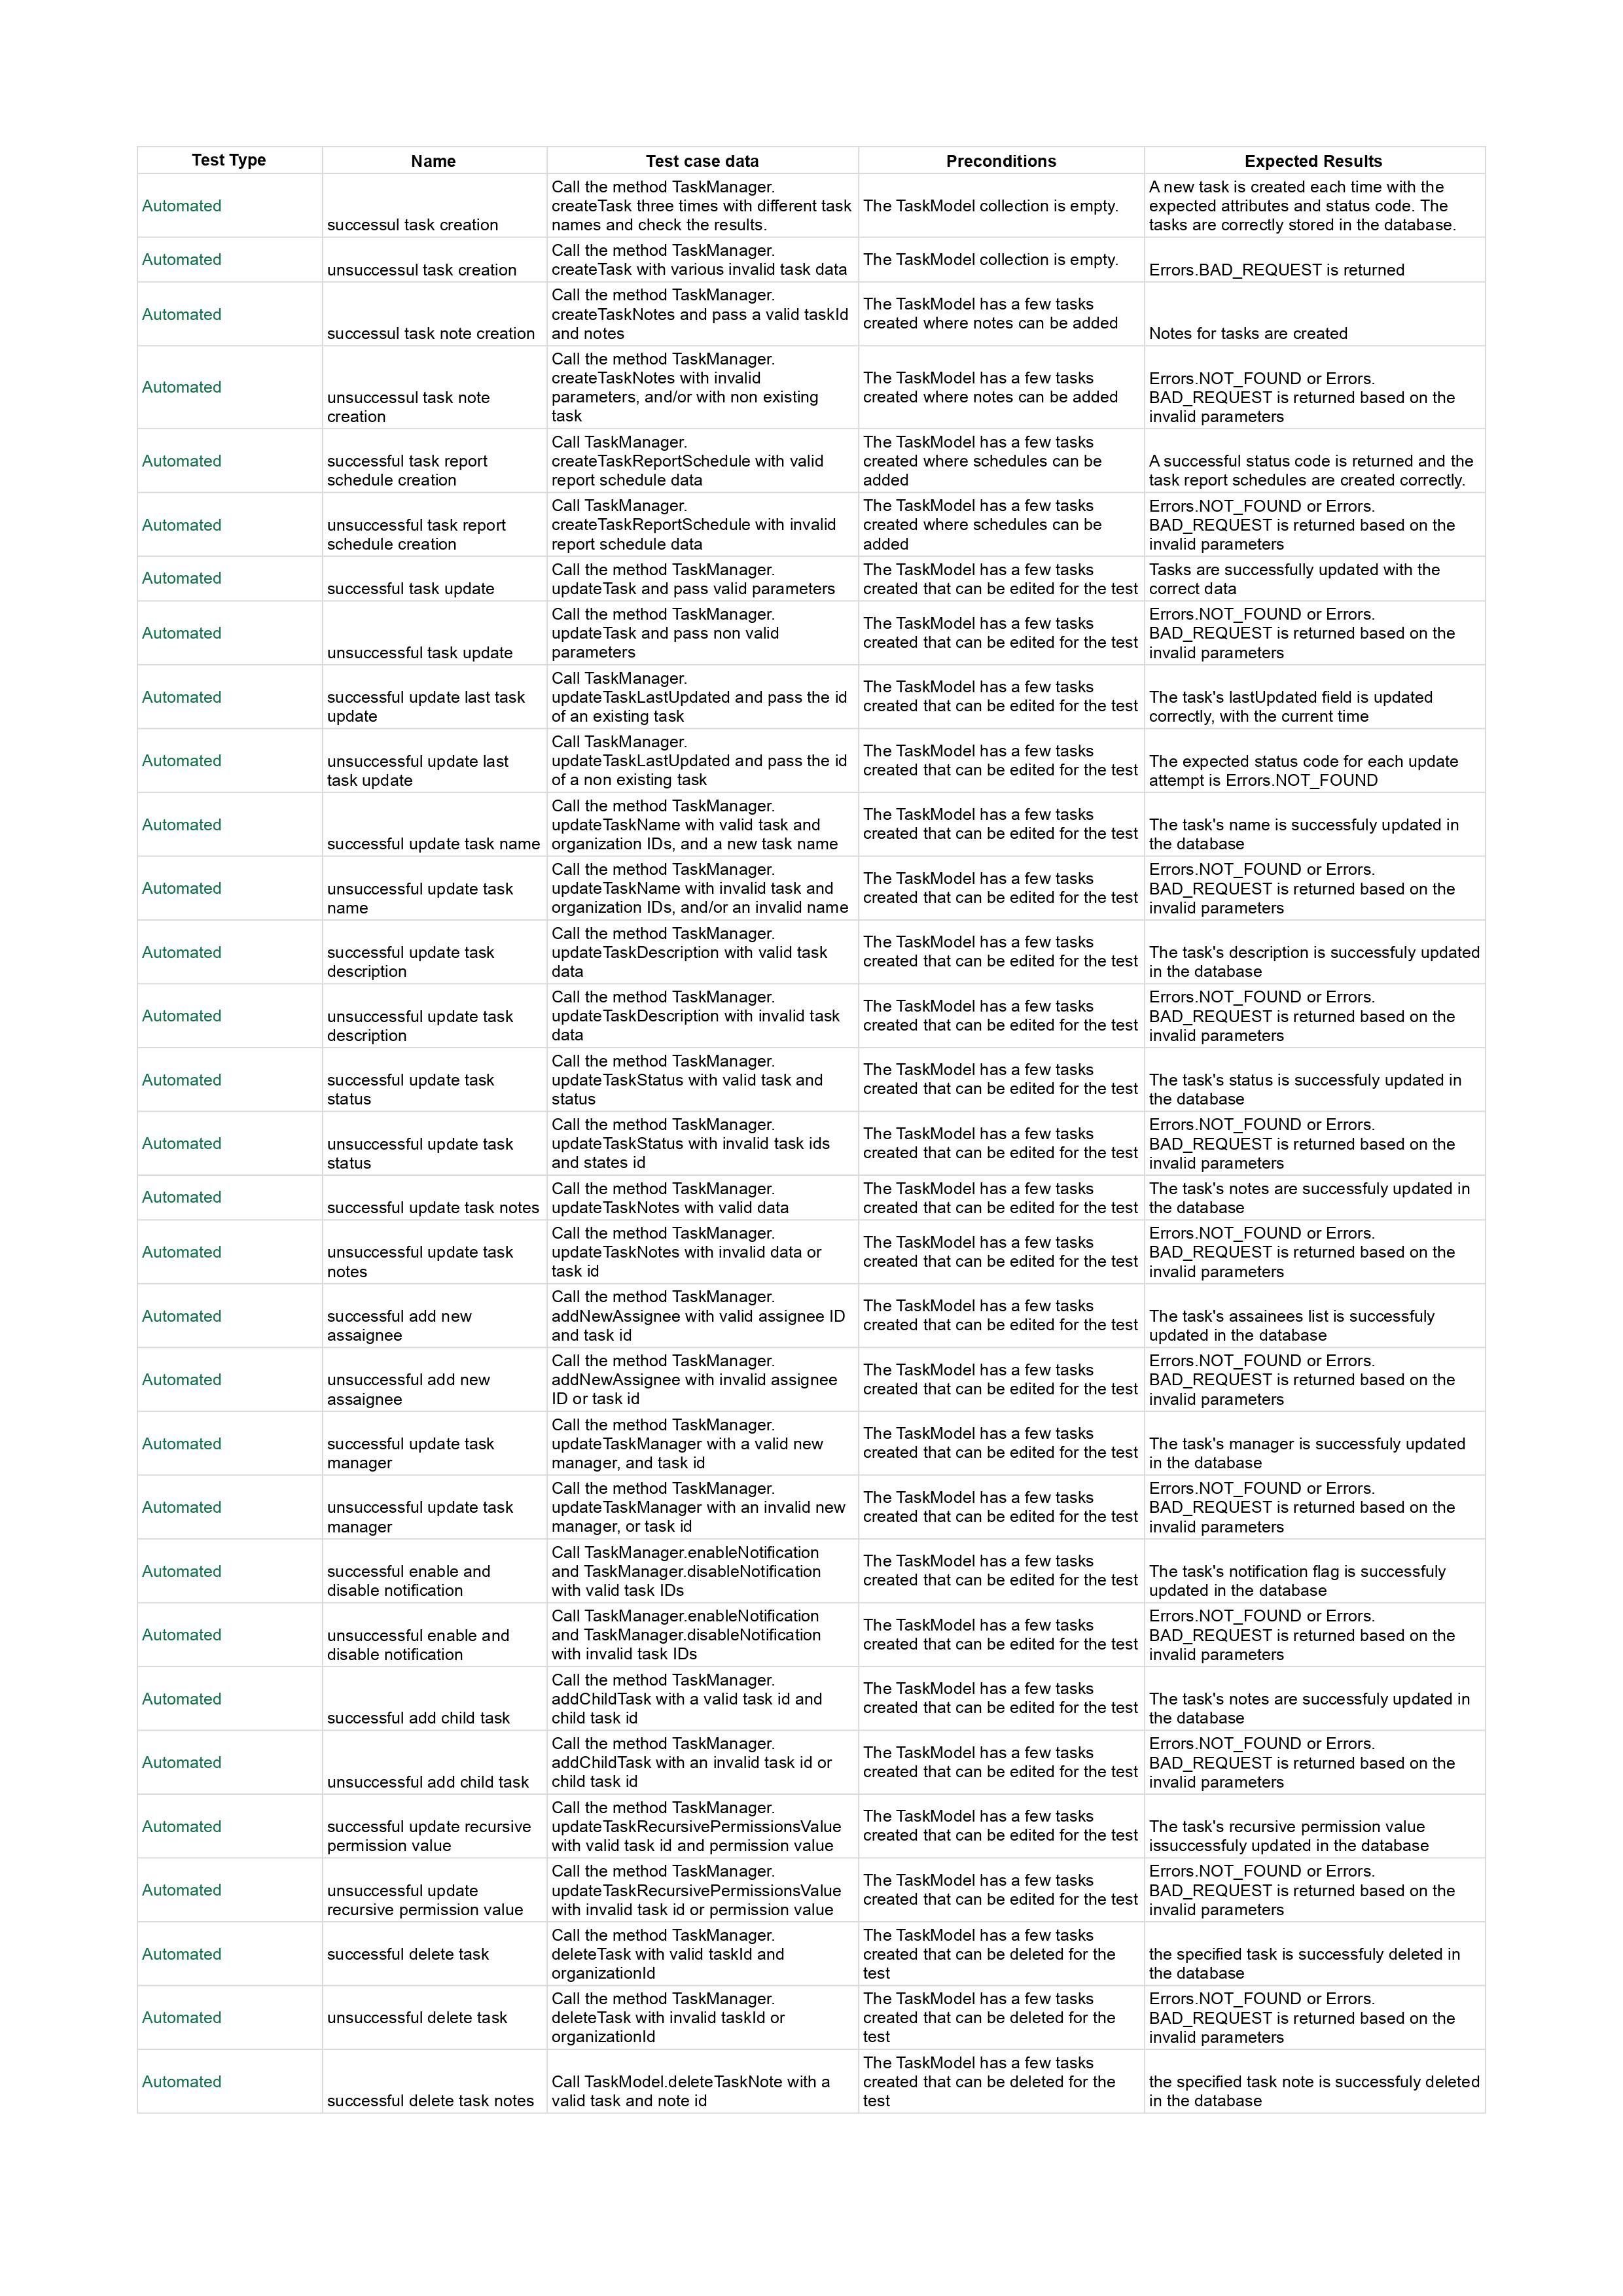
\includegraphics[width=0.95\textwidth]{images/Test_DatabaseManagerTaskManager-immagini-0.jpg}
\newline
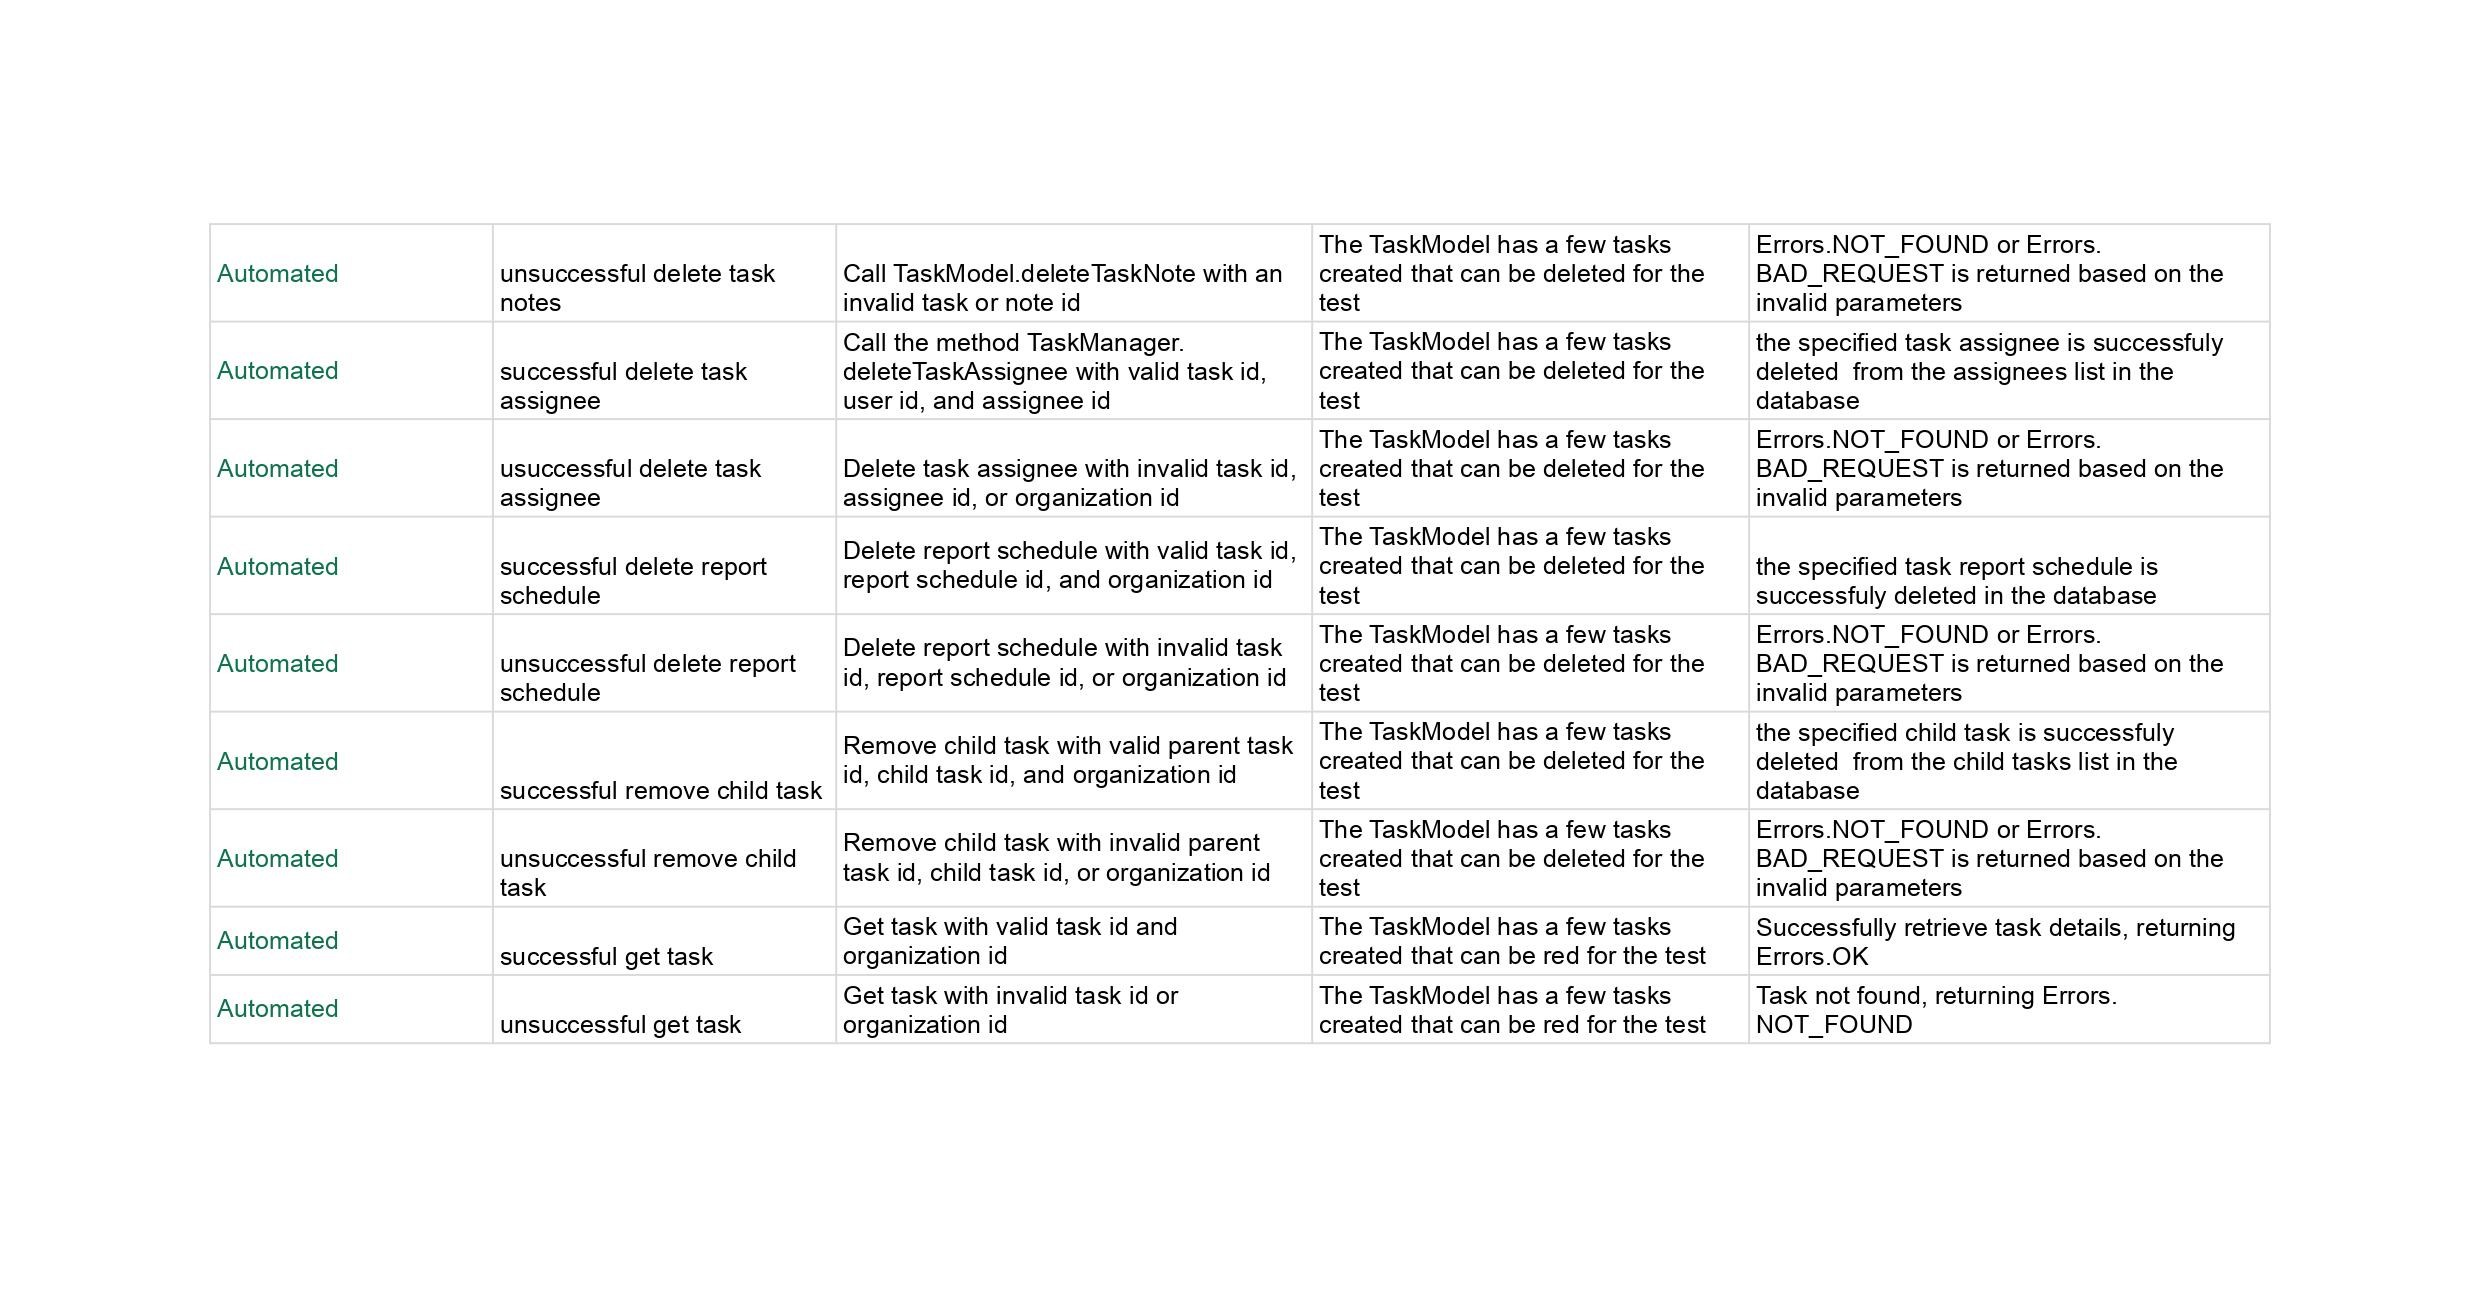
\includegraphics[width=0.95\textwidth]{images/Test_DatabaseManagerTaskManager-immagini-1.jpg}
\subsection*{Test OrganizationManager}
This section is dedicated to the tests for the OrganizationManager class, which is responsible for managing organizations in the database, with the integrated API.
\newline
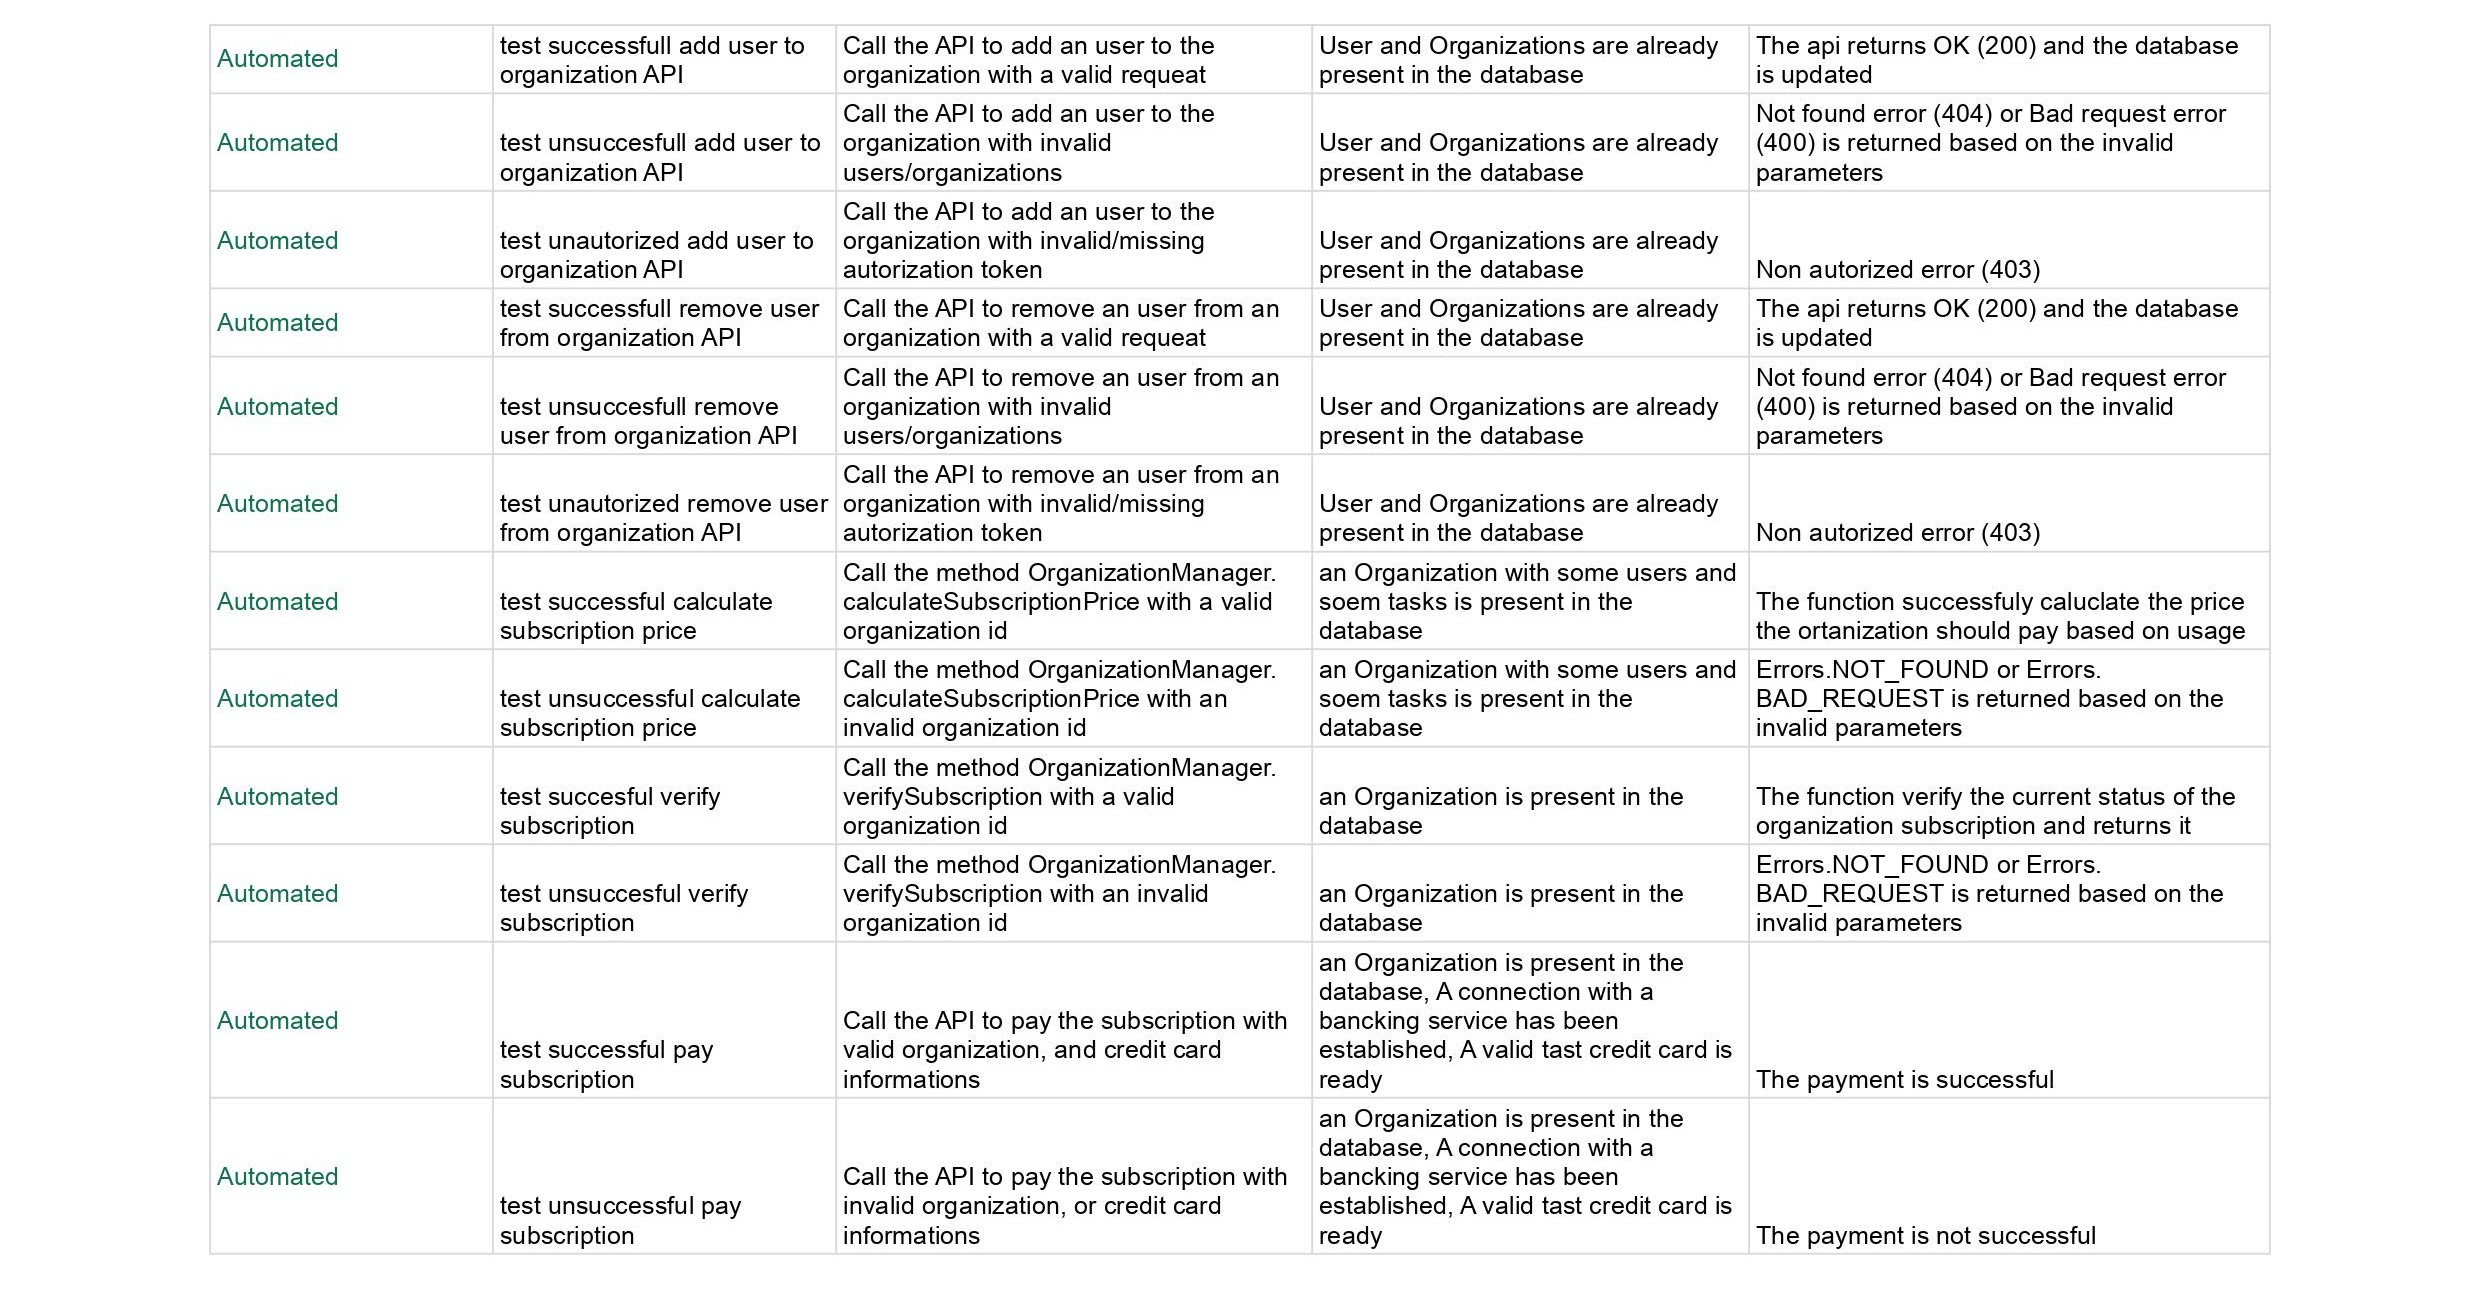
\includegraphics[width=0.95\textwidth]{images/Test_OrganizationManager.jpg}

\subsection*{Test Report Page}
This section includes manual tests for the Report Page, which is responsible for generating reports.
\newline
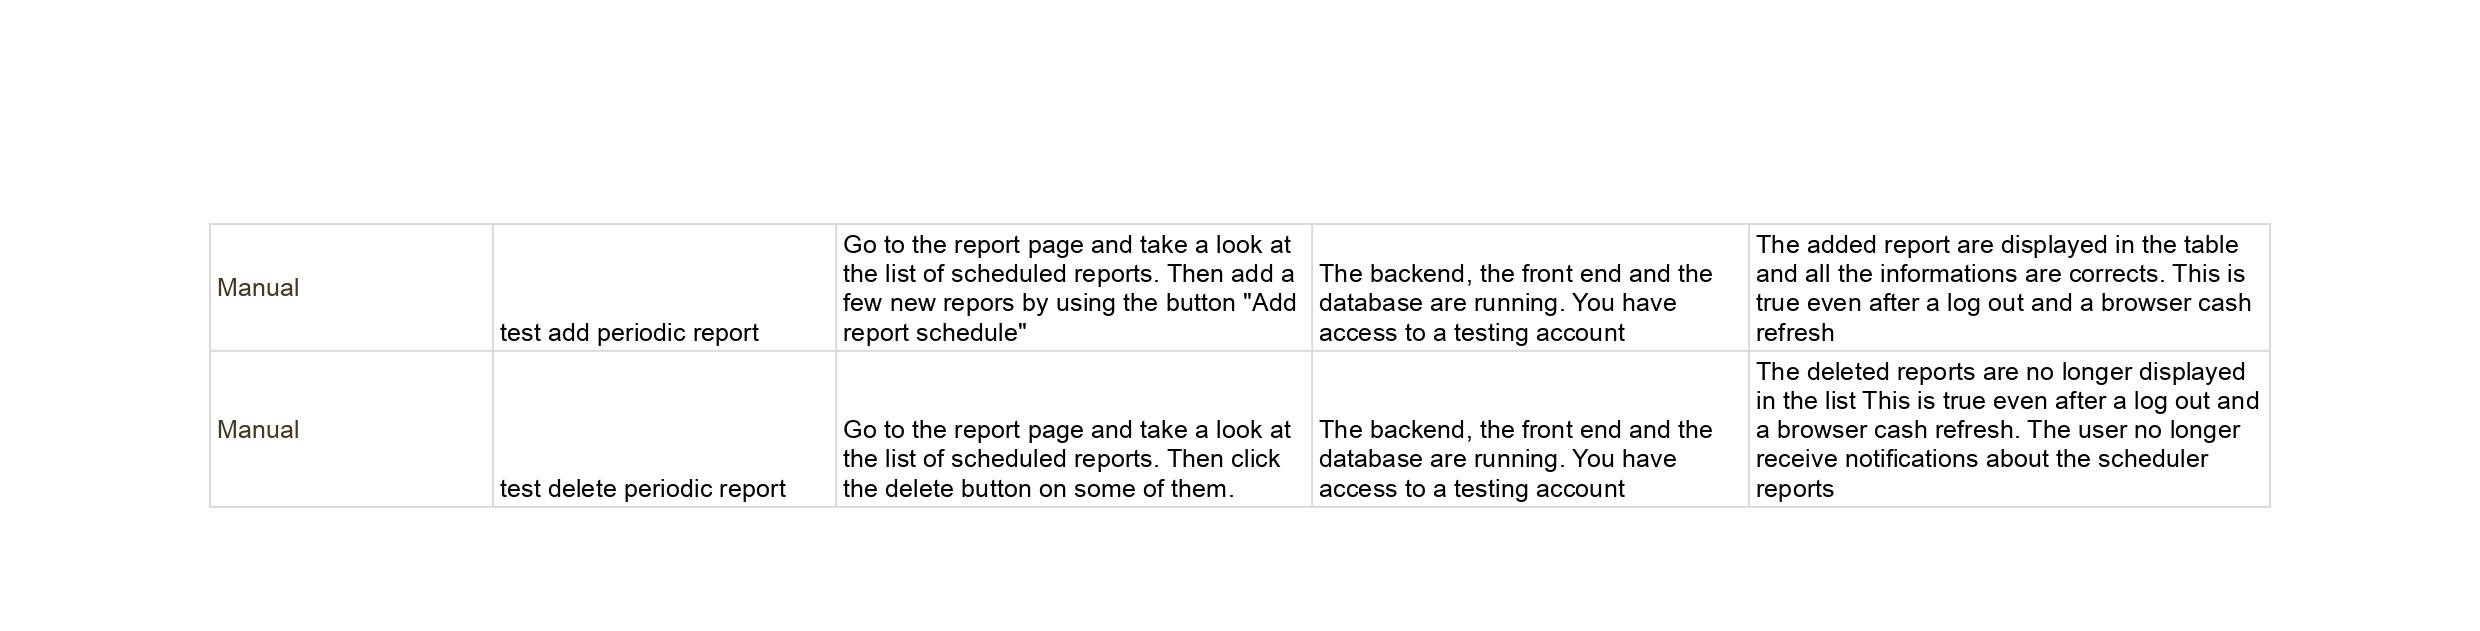
\includegraphics[width=0.95\textwidth]{images/Test_ReportPage.jpg}
\subsection*{Test NotificationManager}
This section includes automated tests for the NotificationManager class, which is responsible for managing notifications in the database.
\newline
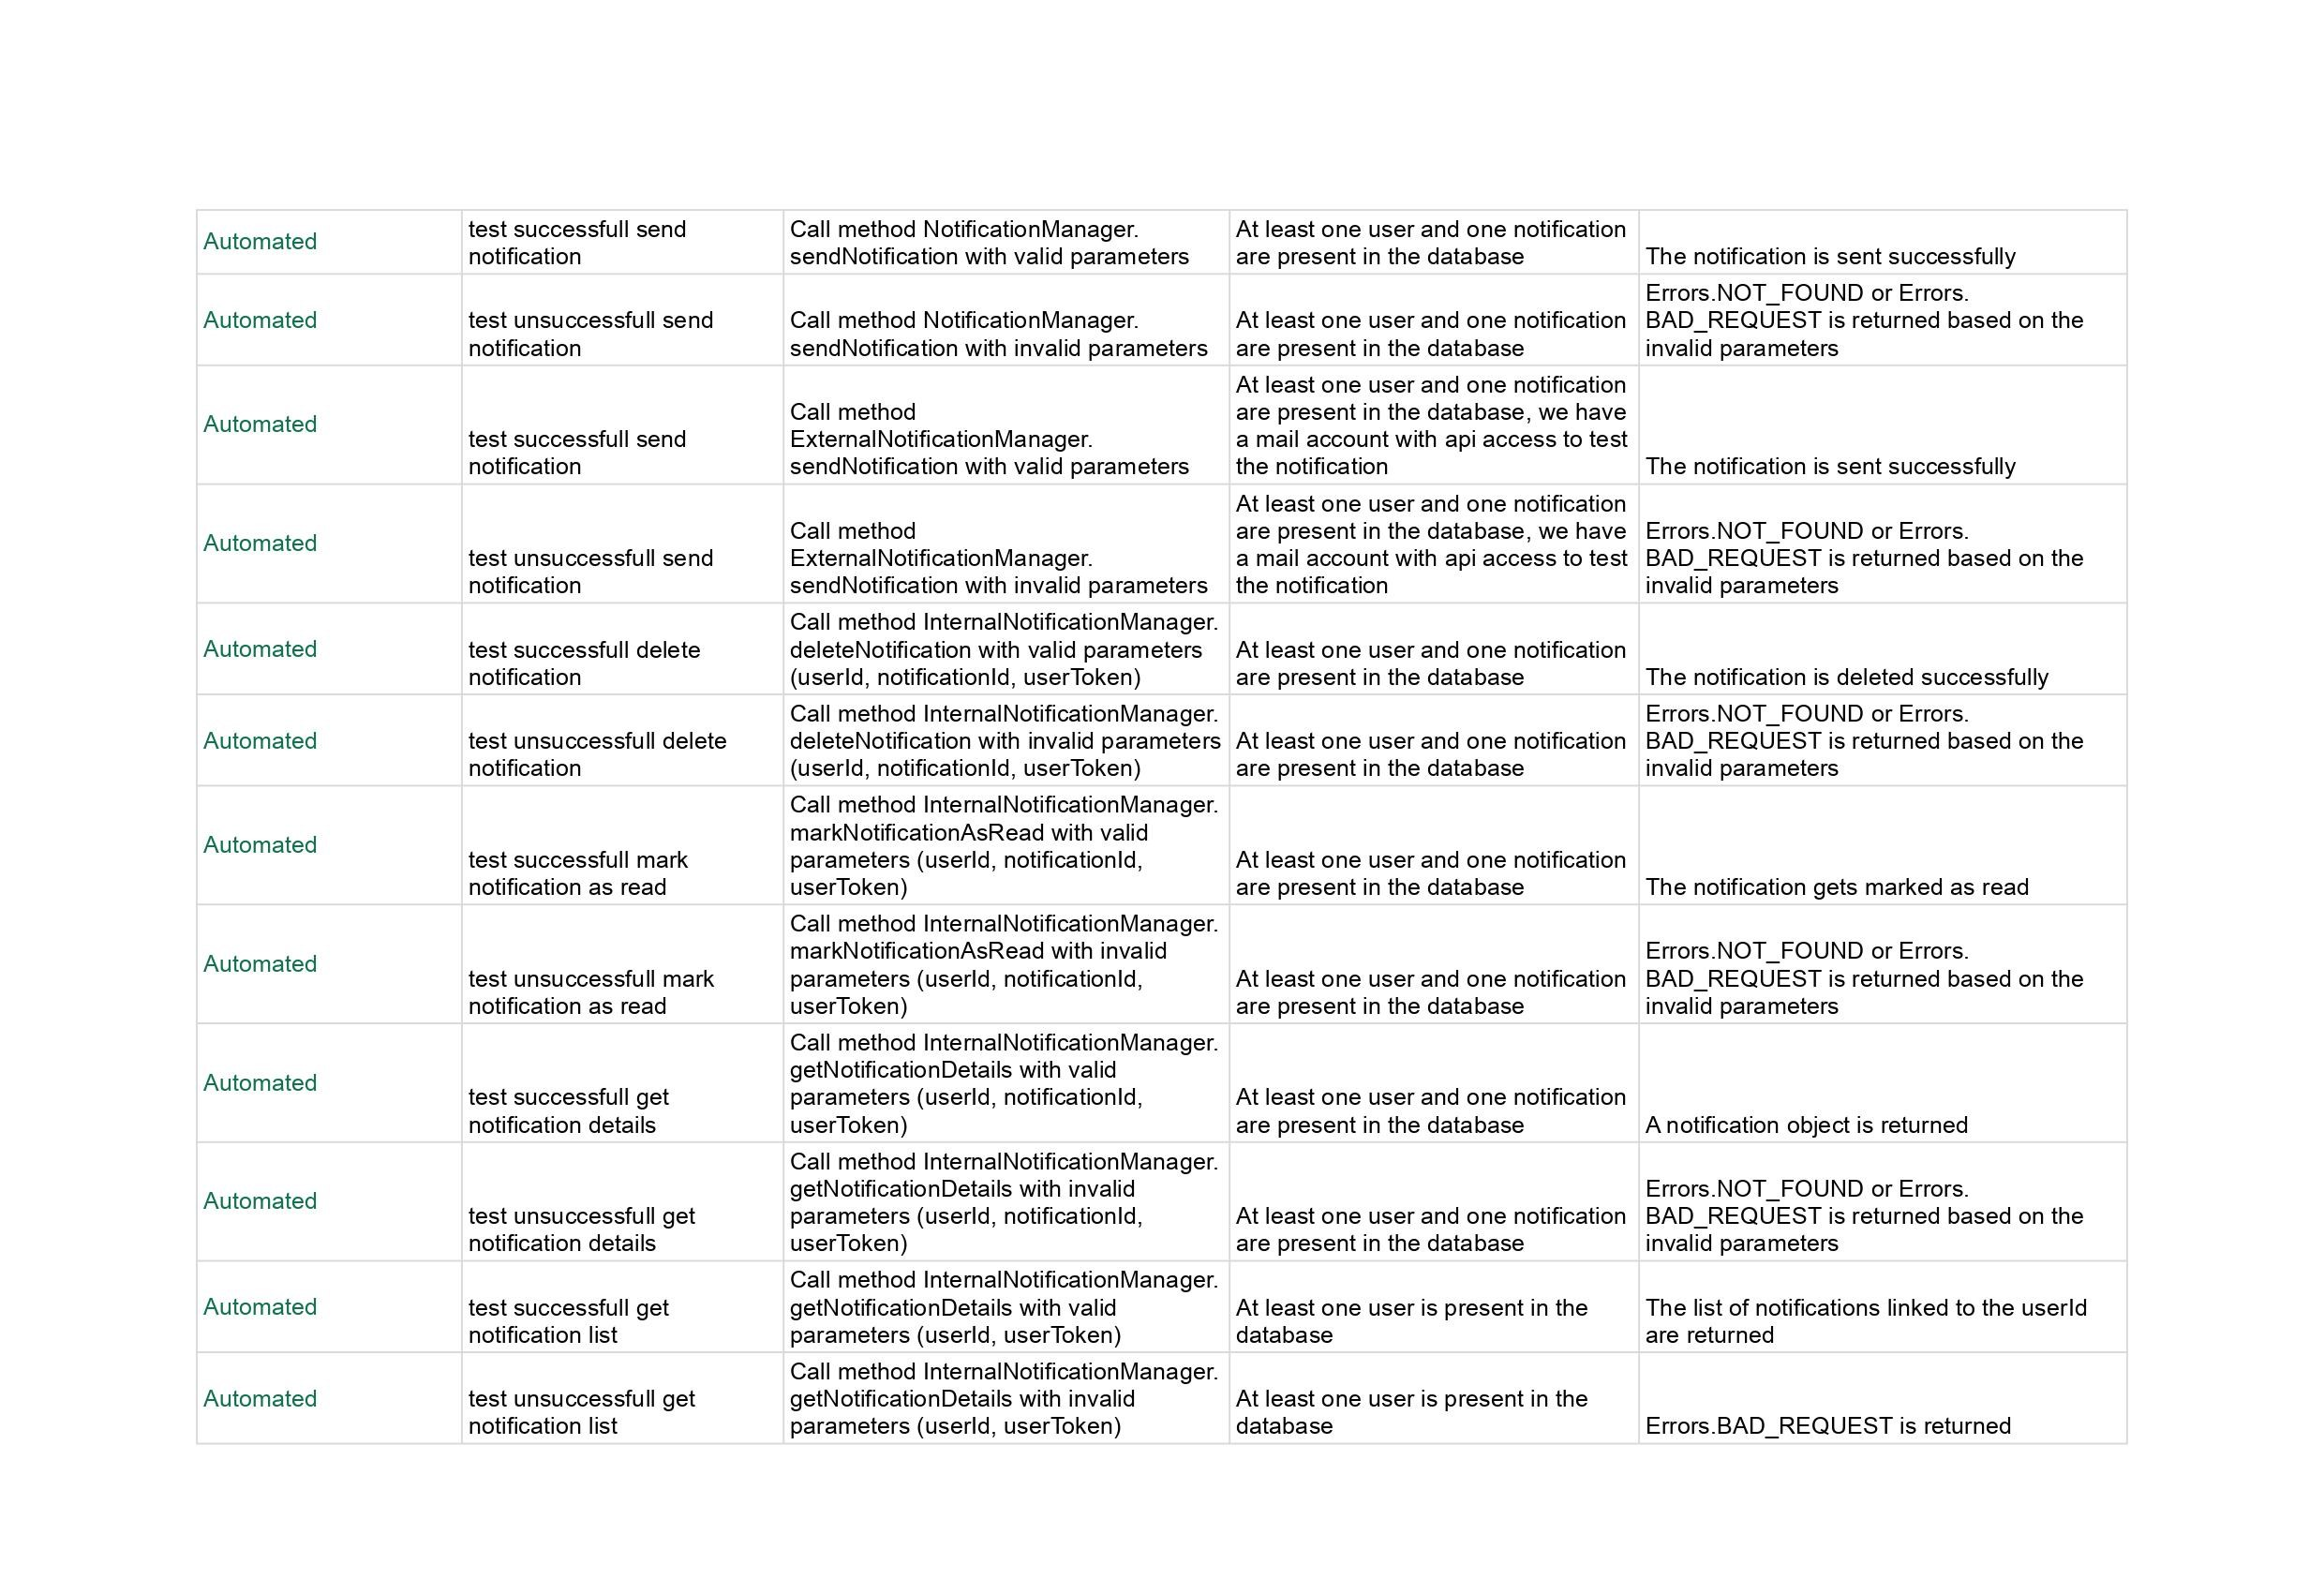
\includegraphics[width=0.95\textwidth]{images/Test_NotificationManager.jpg}

\subsection*{Test ReportManager}
This section includes automated tests for the ReportManager class, which is responsible for managing reports in the database.
\newline
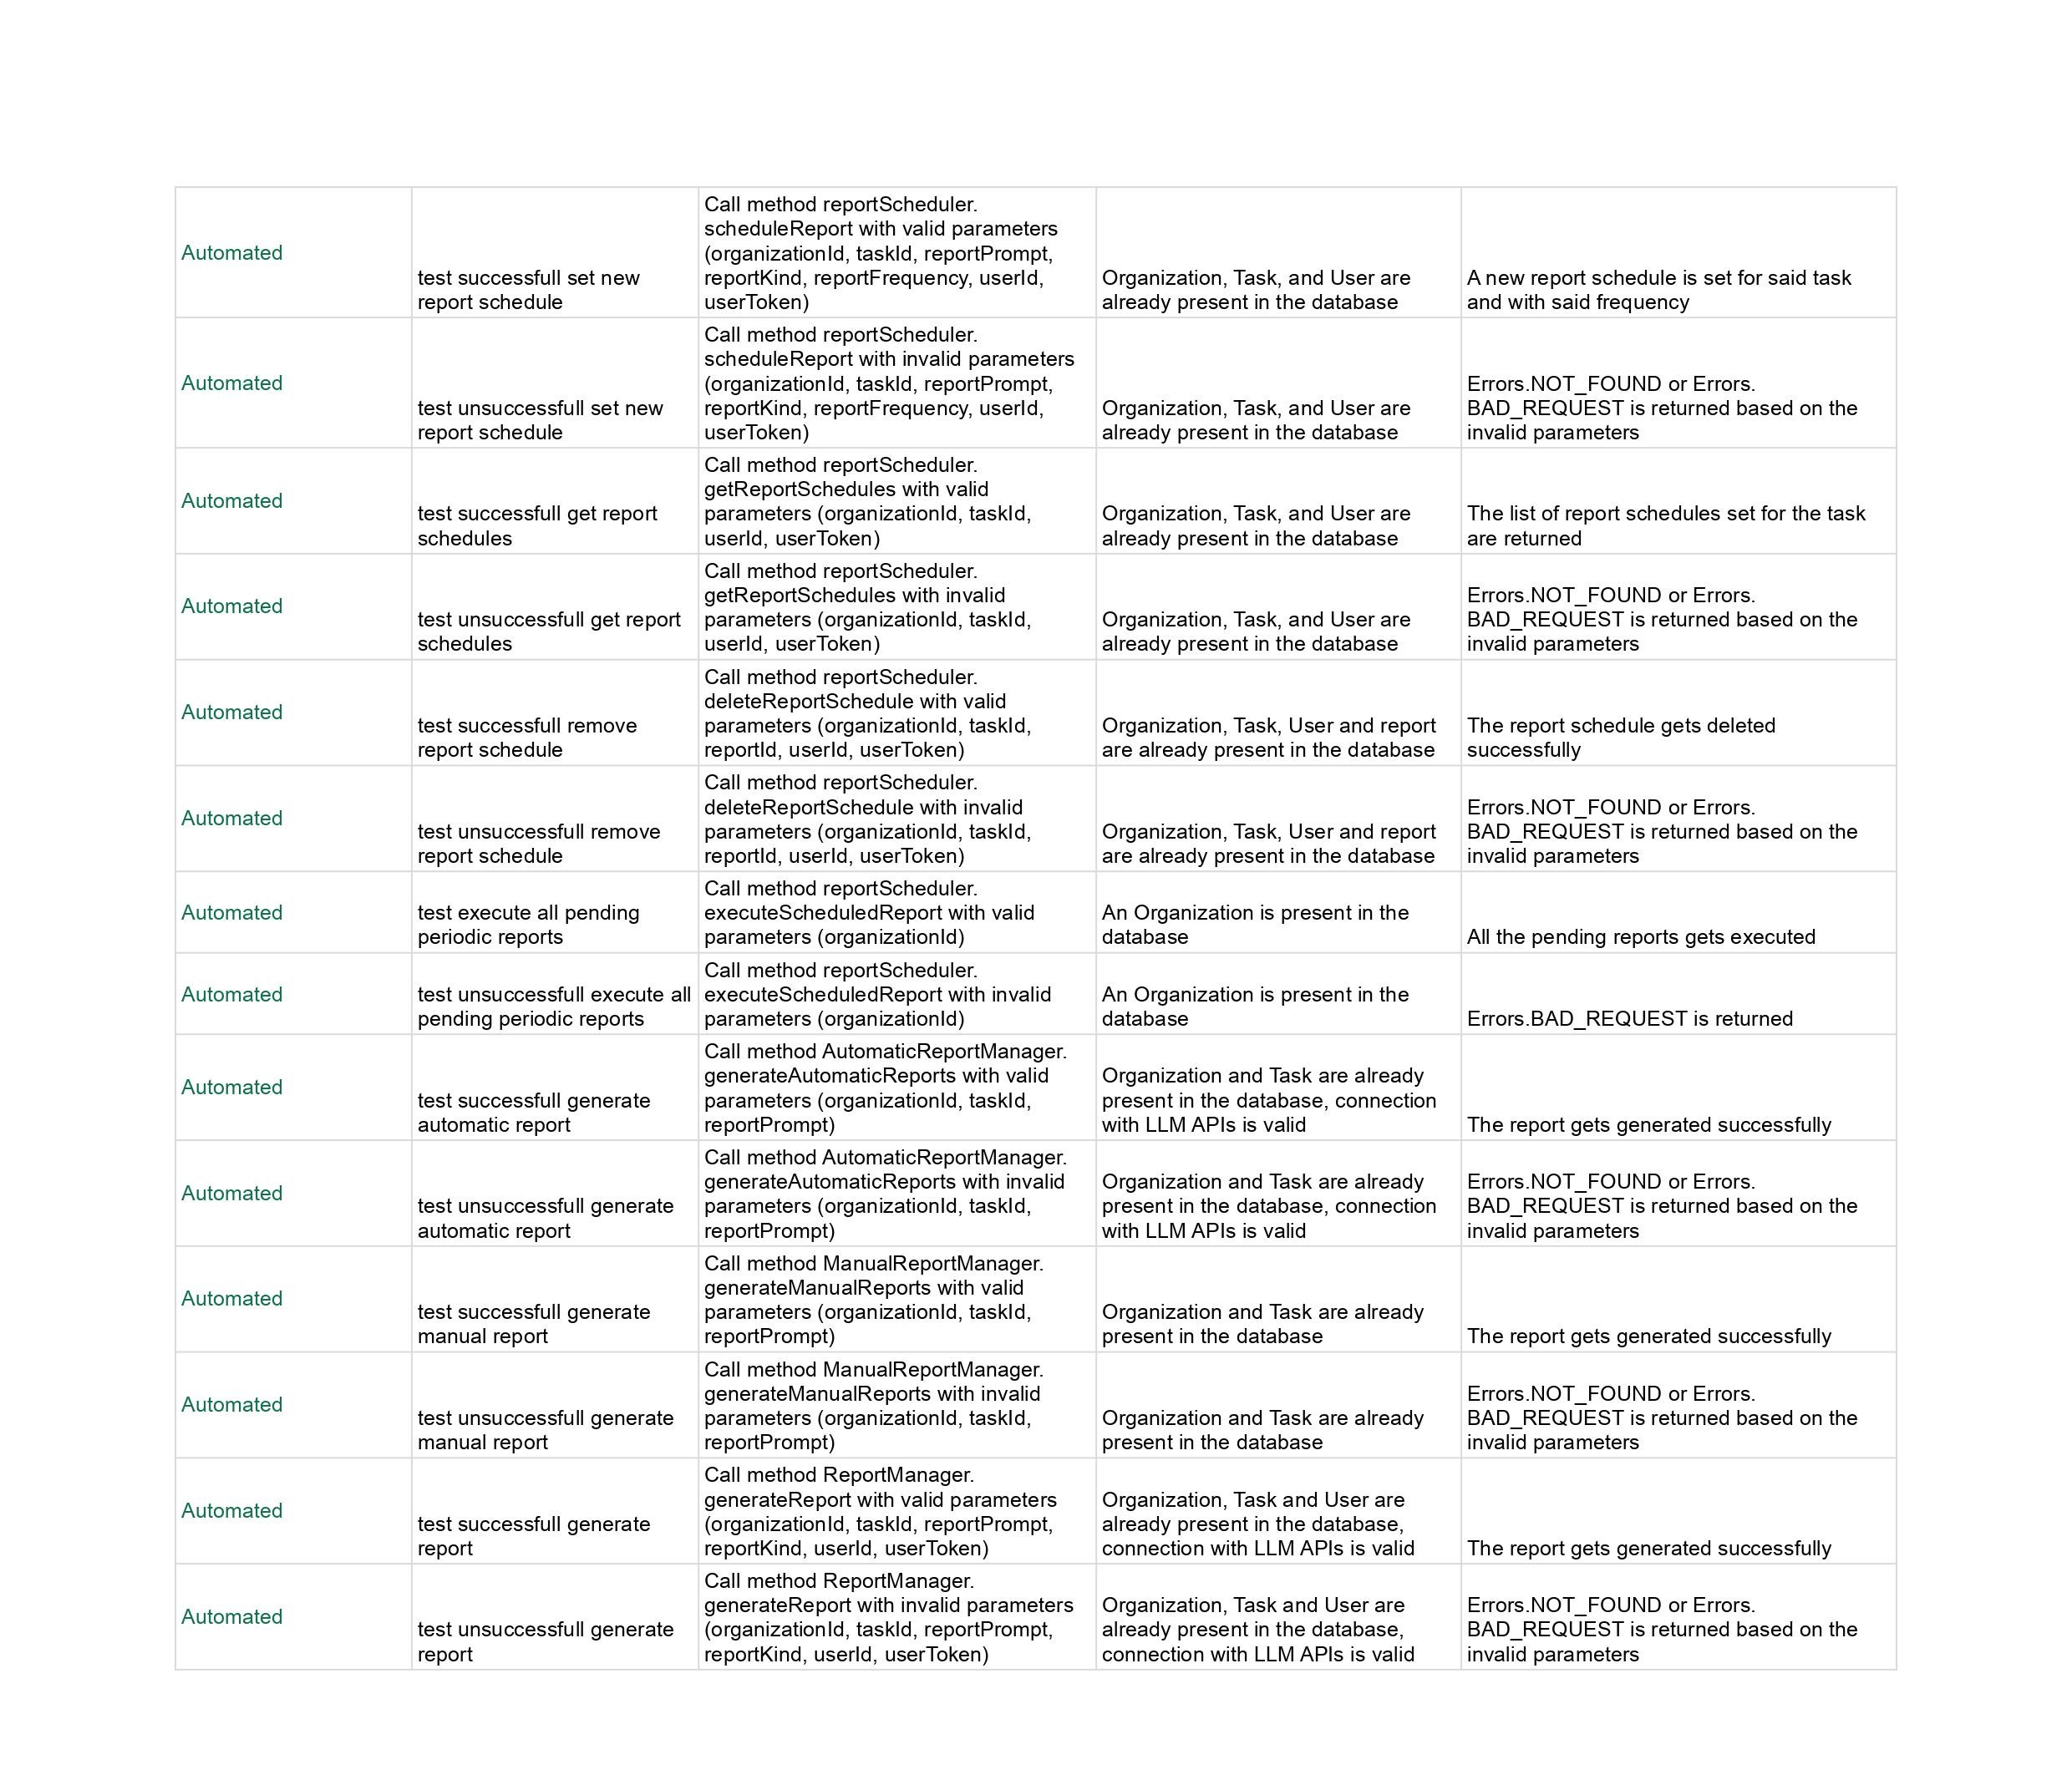
\includegraphics[width=0.95\textwidth]{images/Test_ReportManager.jpg}

\subsection*{Test DatabaseManager::OrganizationManager}
This section is dedicated to the tests for the OrganizationManager class, which is responsible for managing organizations in the database.
\newline
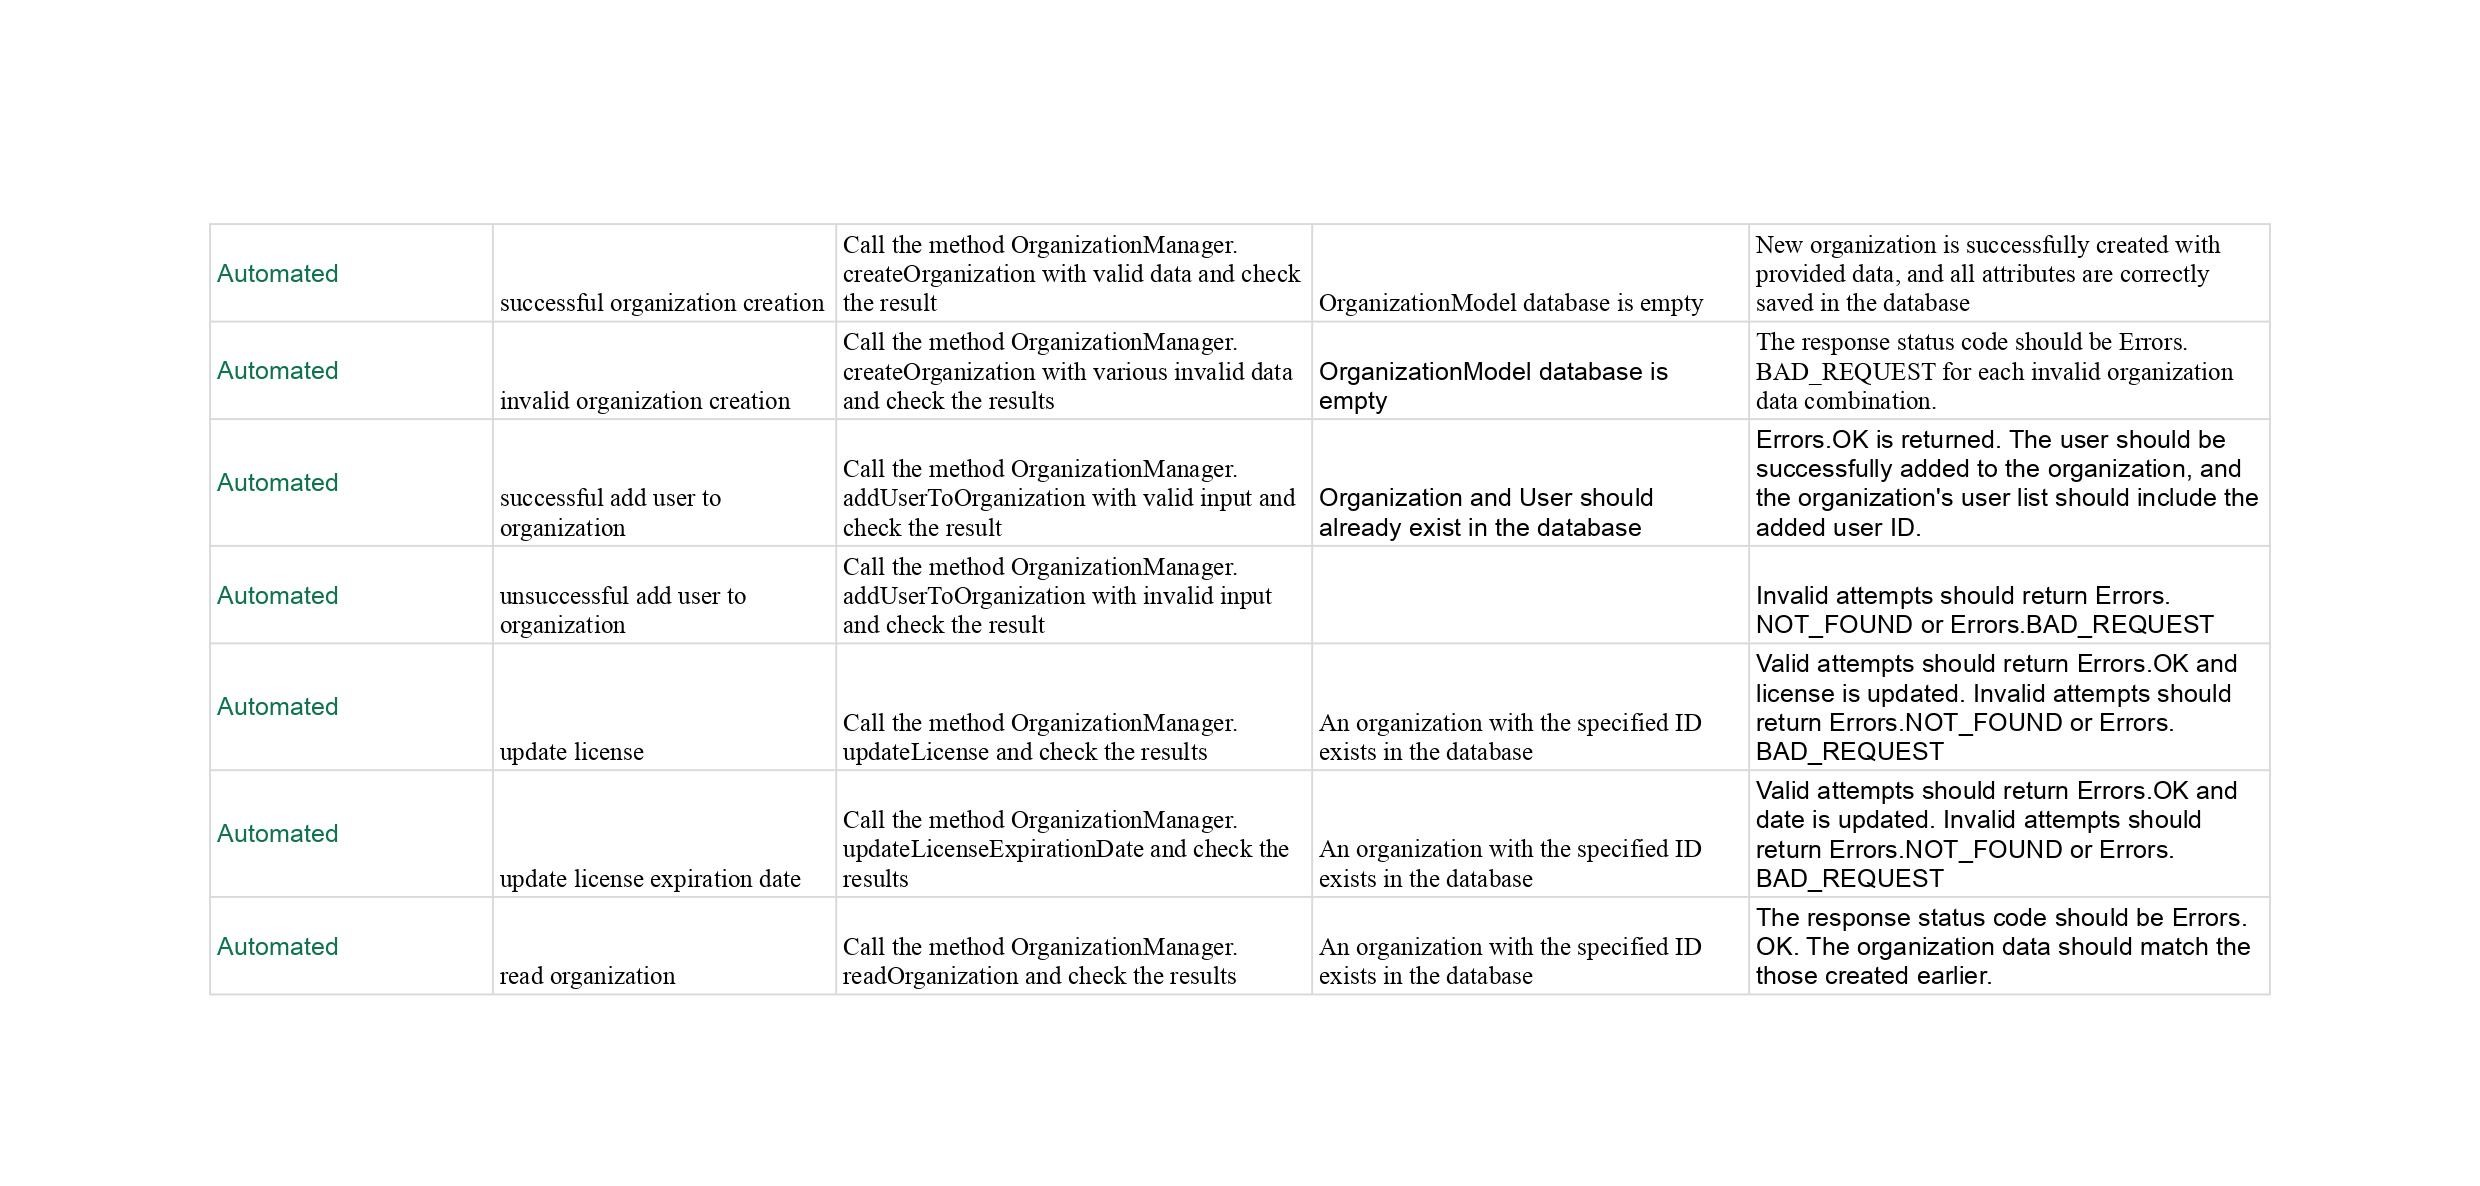
\includegraphics[width=0.95\textwidth]{images/Test_DatabaseManagerOrganizationManager.jpg}

\subsection*{Test AccountManager}
This section includes automated tests for the AccountManager class, which is responsible for managing accounts in the database.
\newline
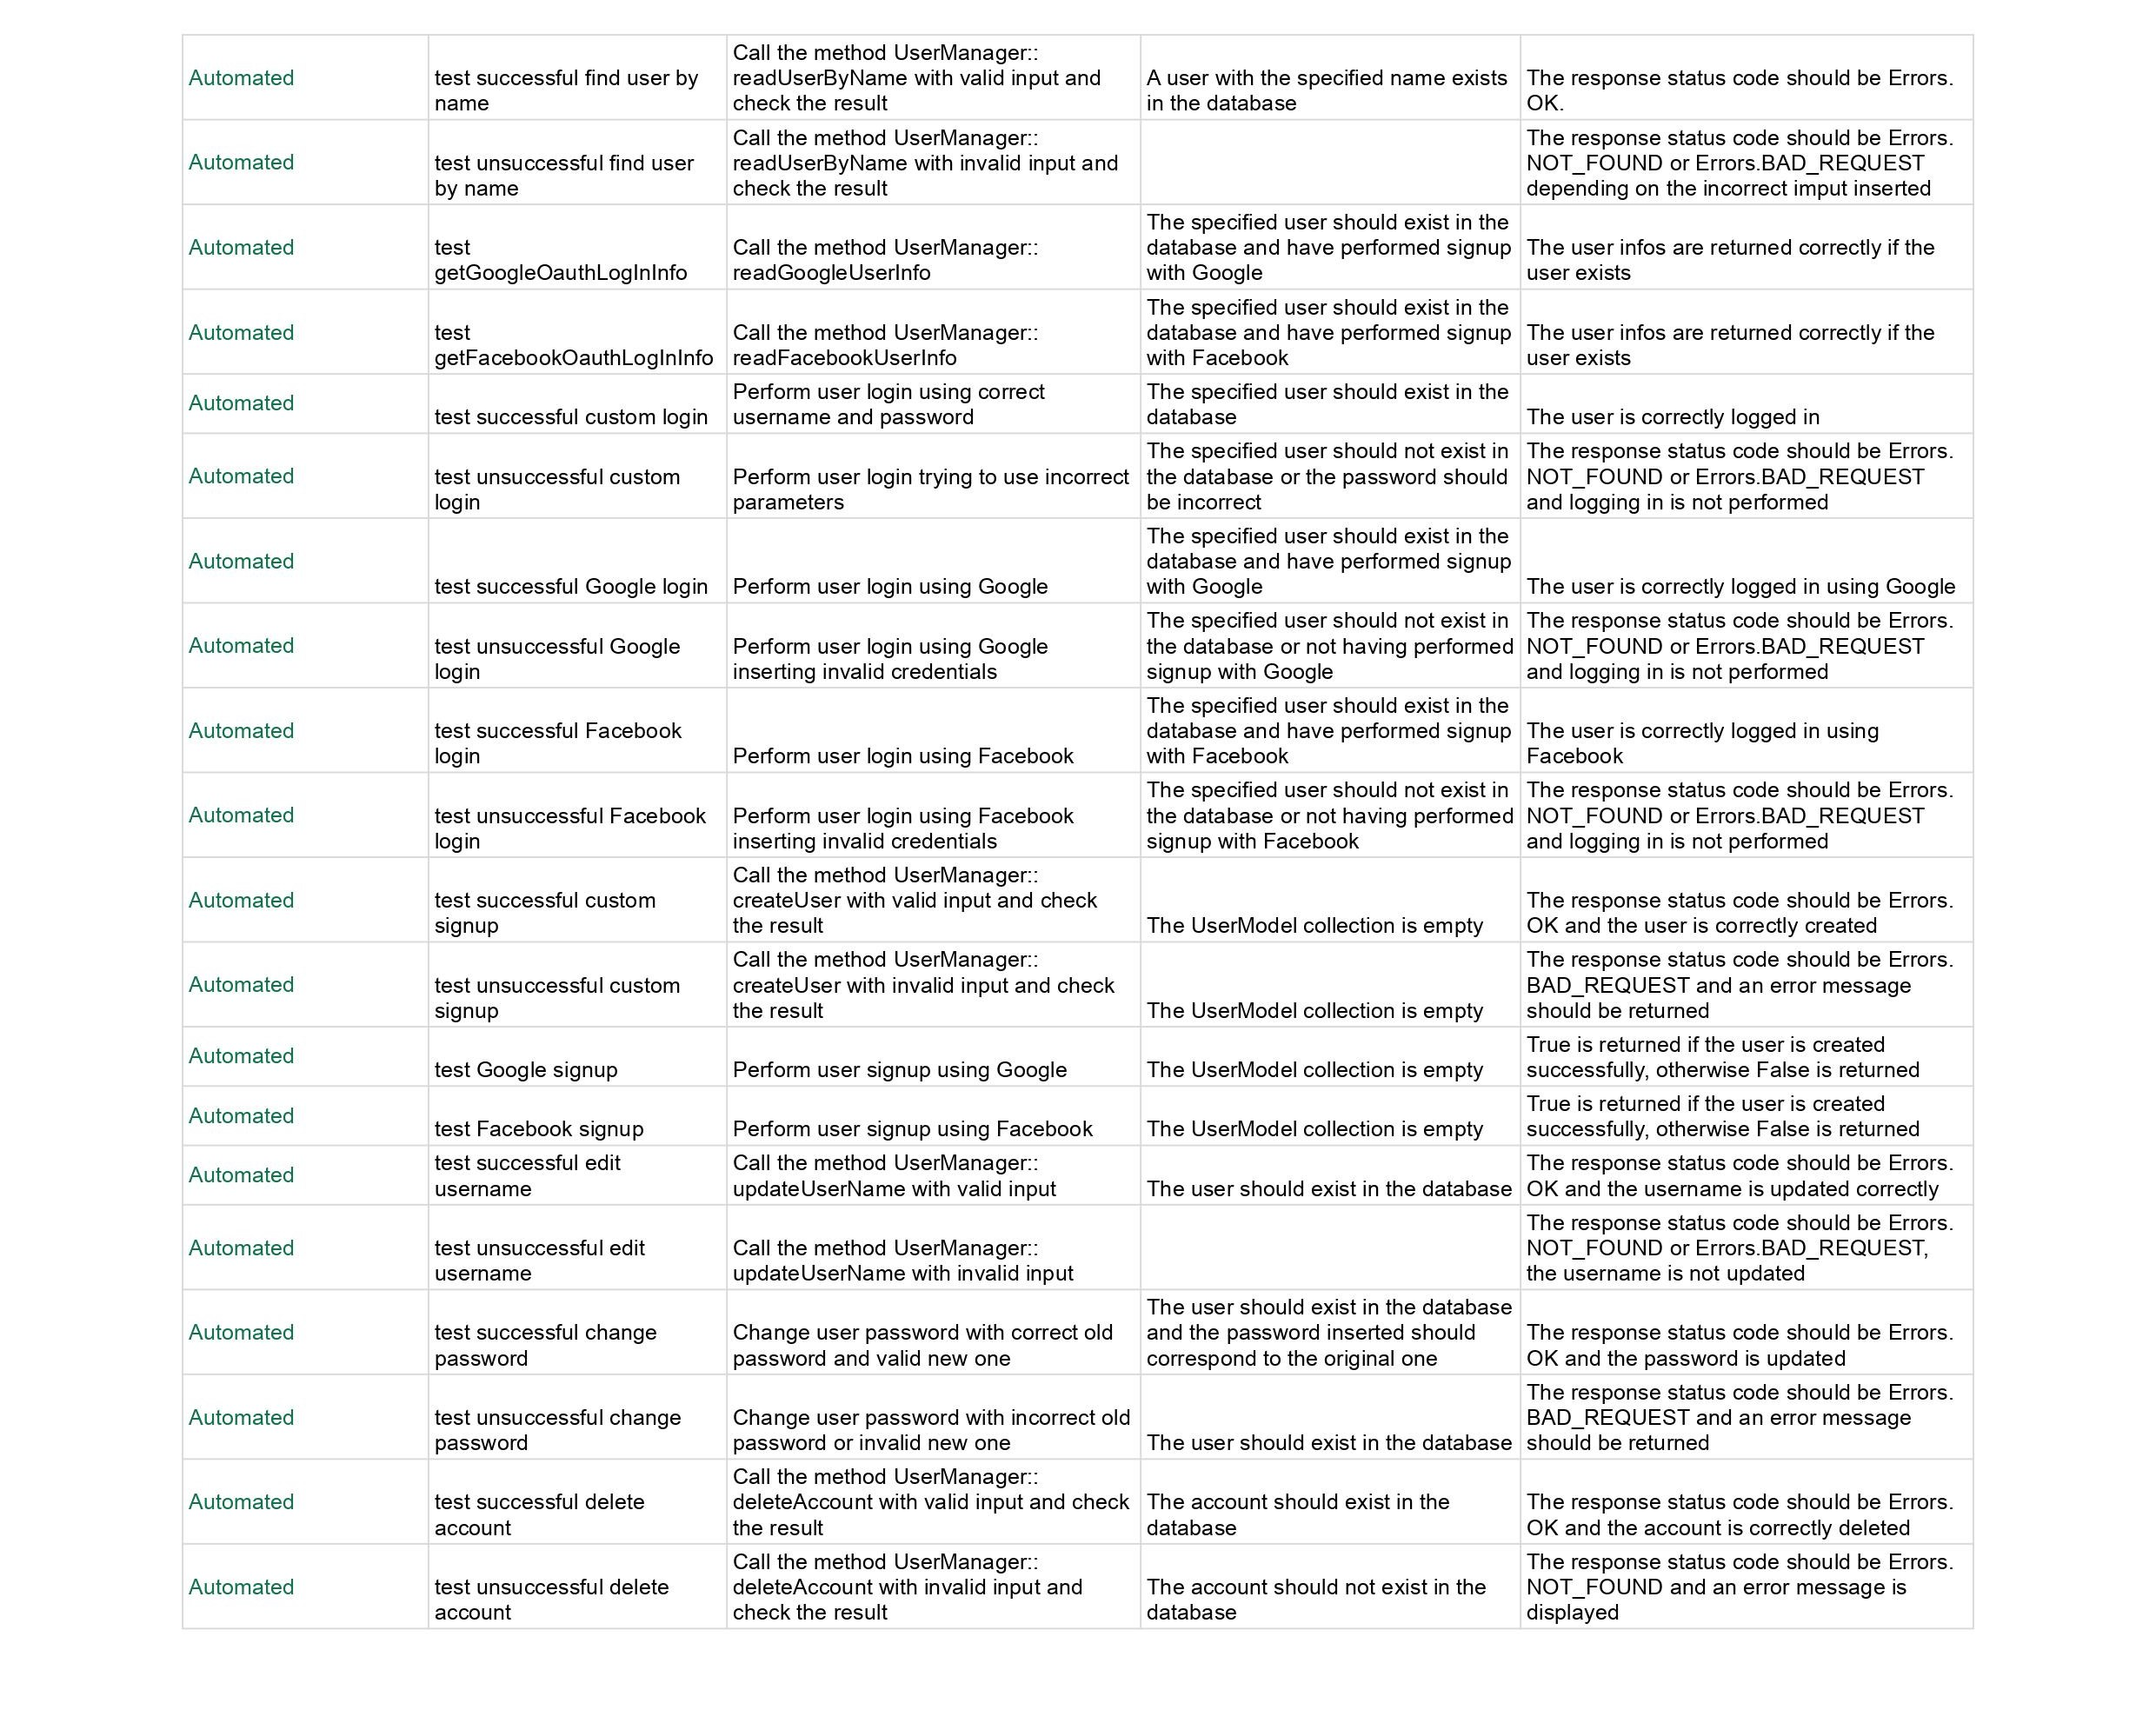
\includegraphics[width=0.95\textwidth]{images/Test_AccountManager.jpg}

\subsection*{Test DatabaseManager::UserManager}
This section is dedicated to the tests for the UserManager class, which is responsible for managing users in the database.
\newline
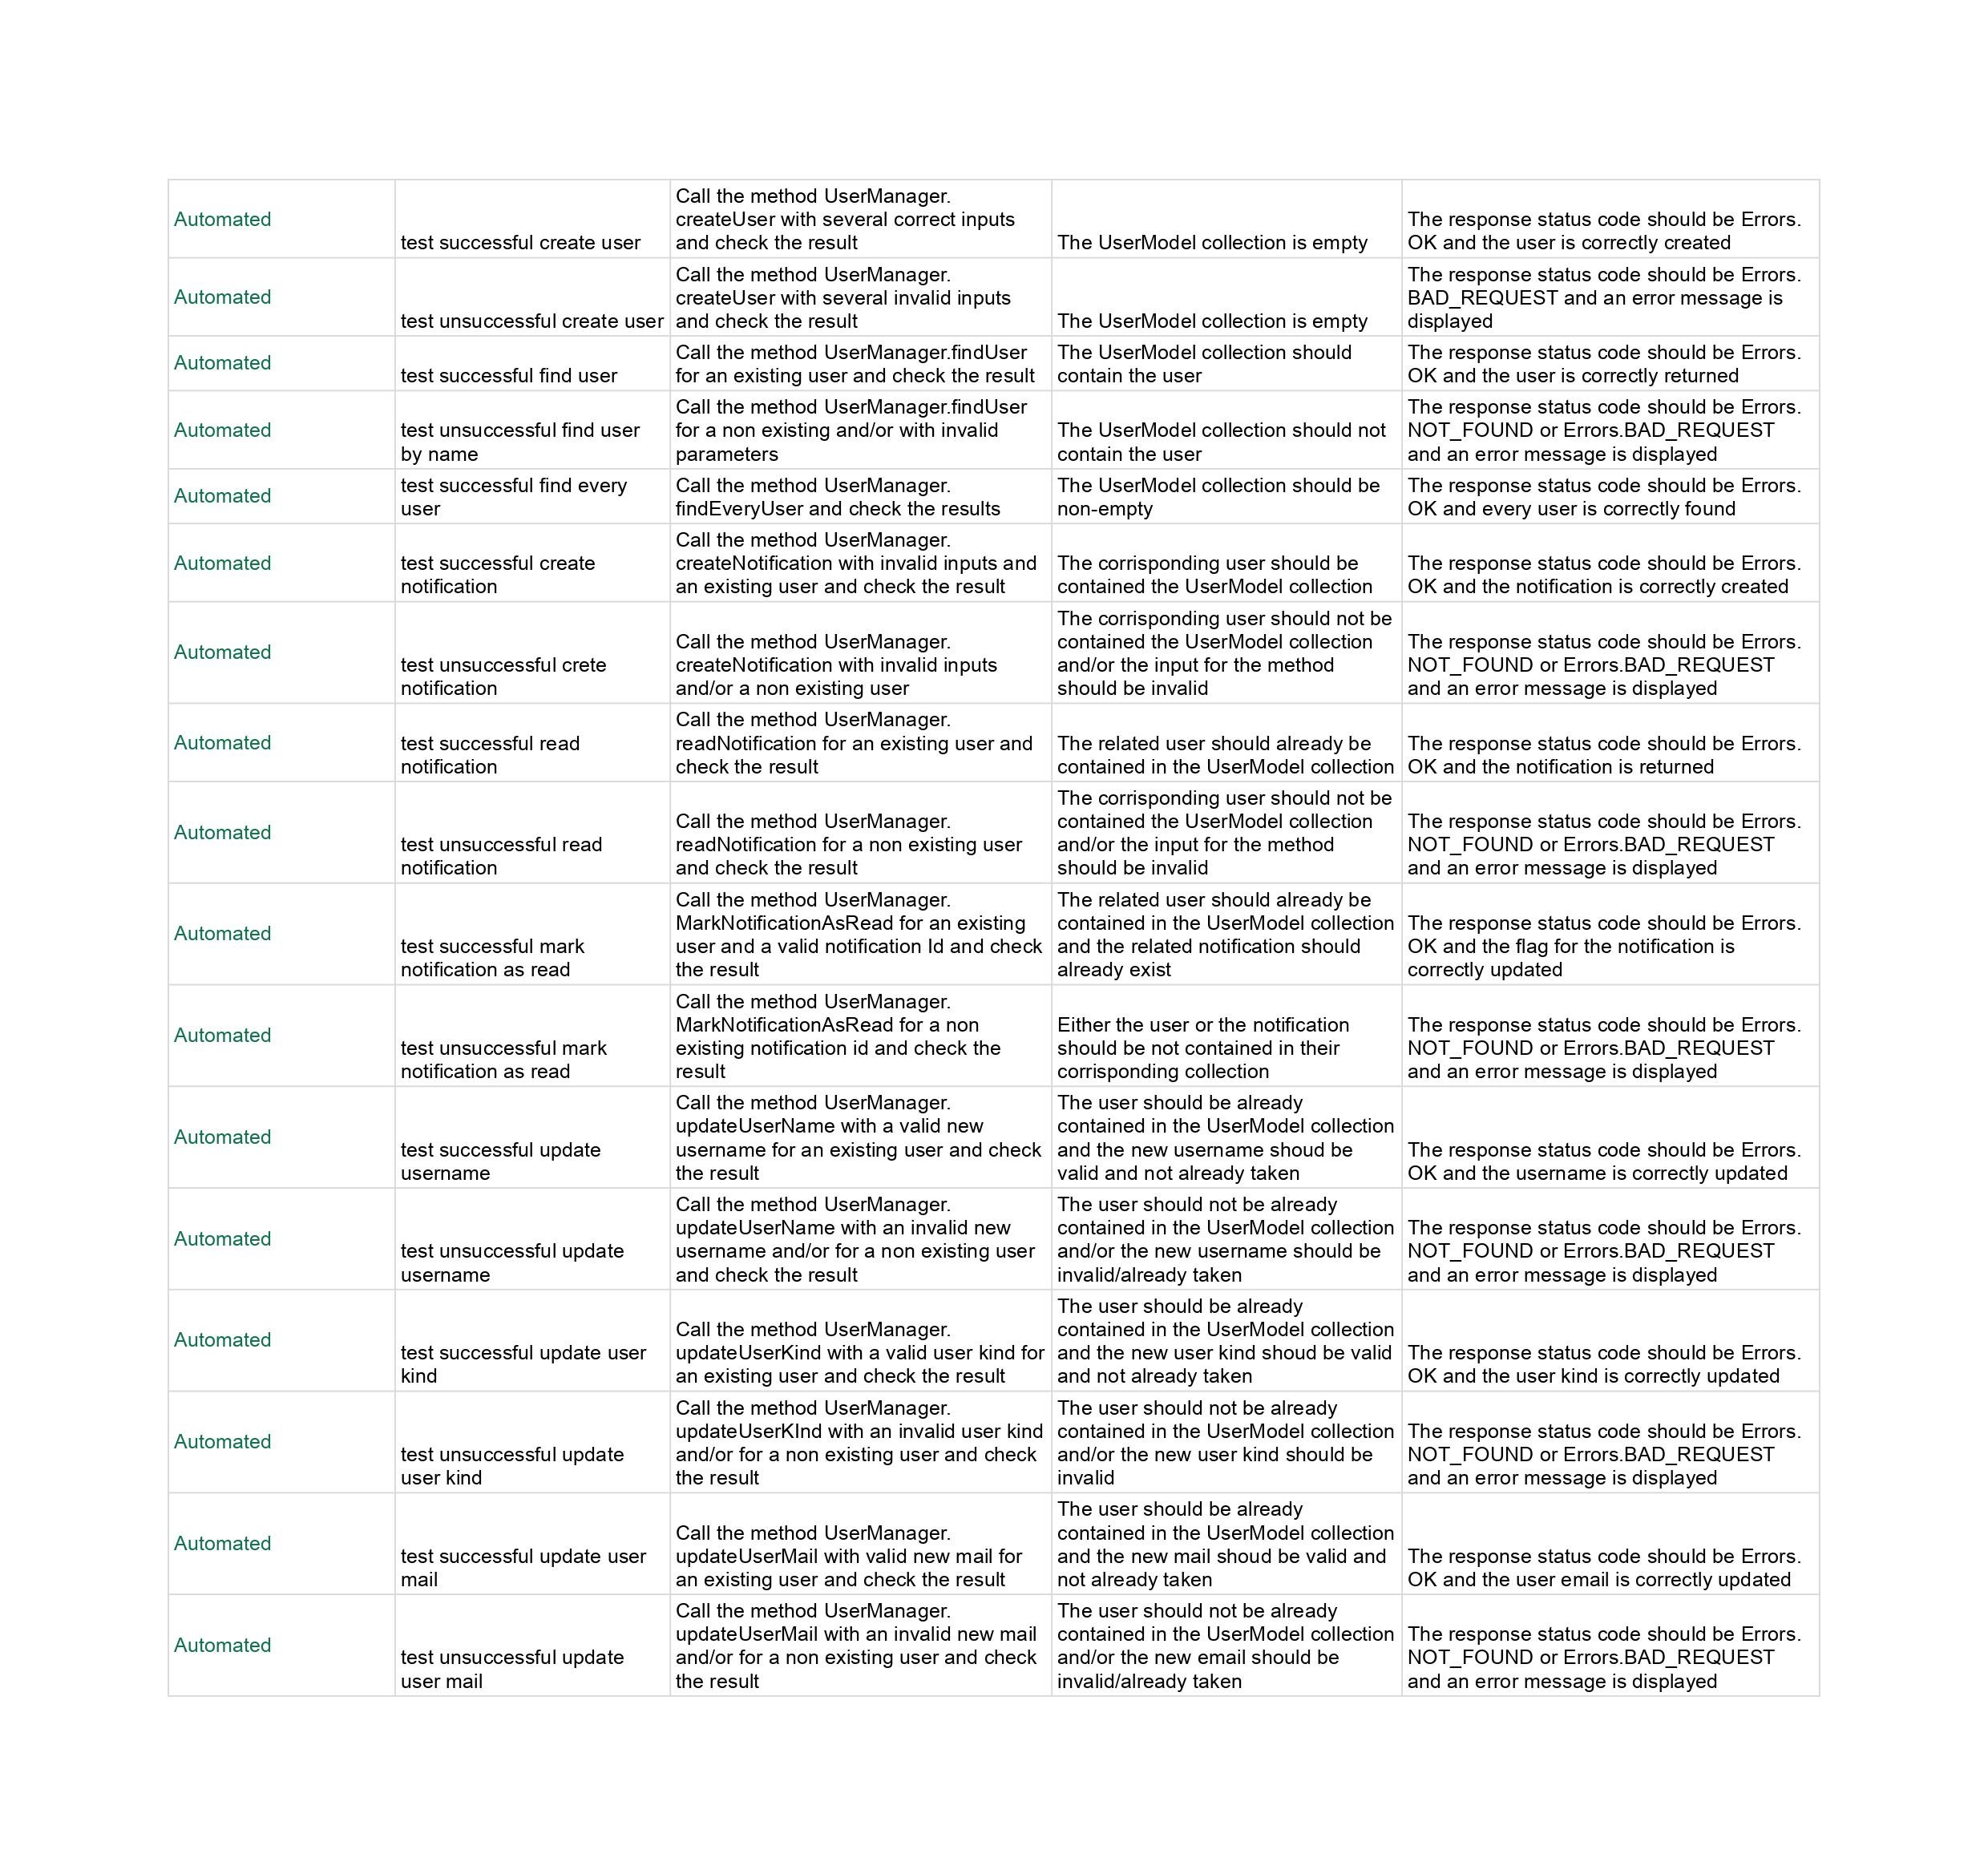
\includegraphics[width=0.95\textwidth]{images/Test_DatabaseManagerUserManager.jpg}

\subsection*{Test TaskManager}
This section includes automated tests for the TaskManager class, which is responsible for managing tasks in the database.
\newline
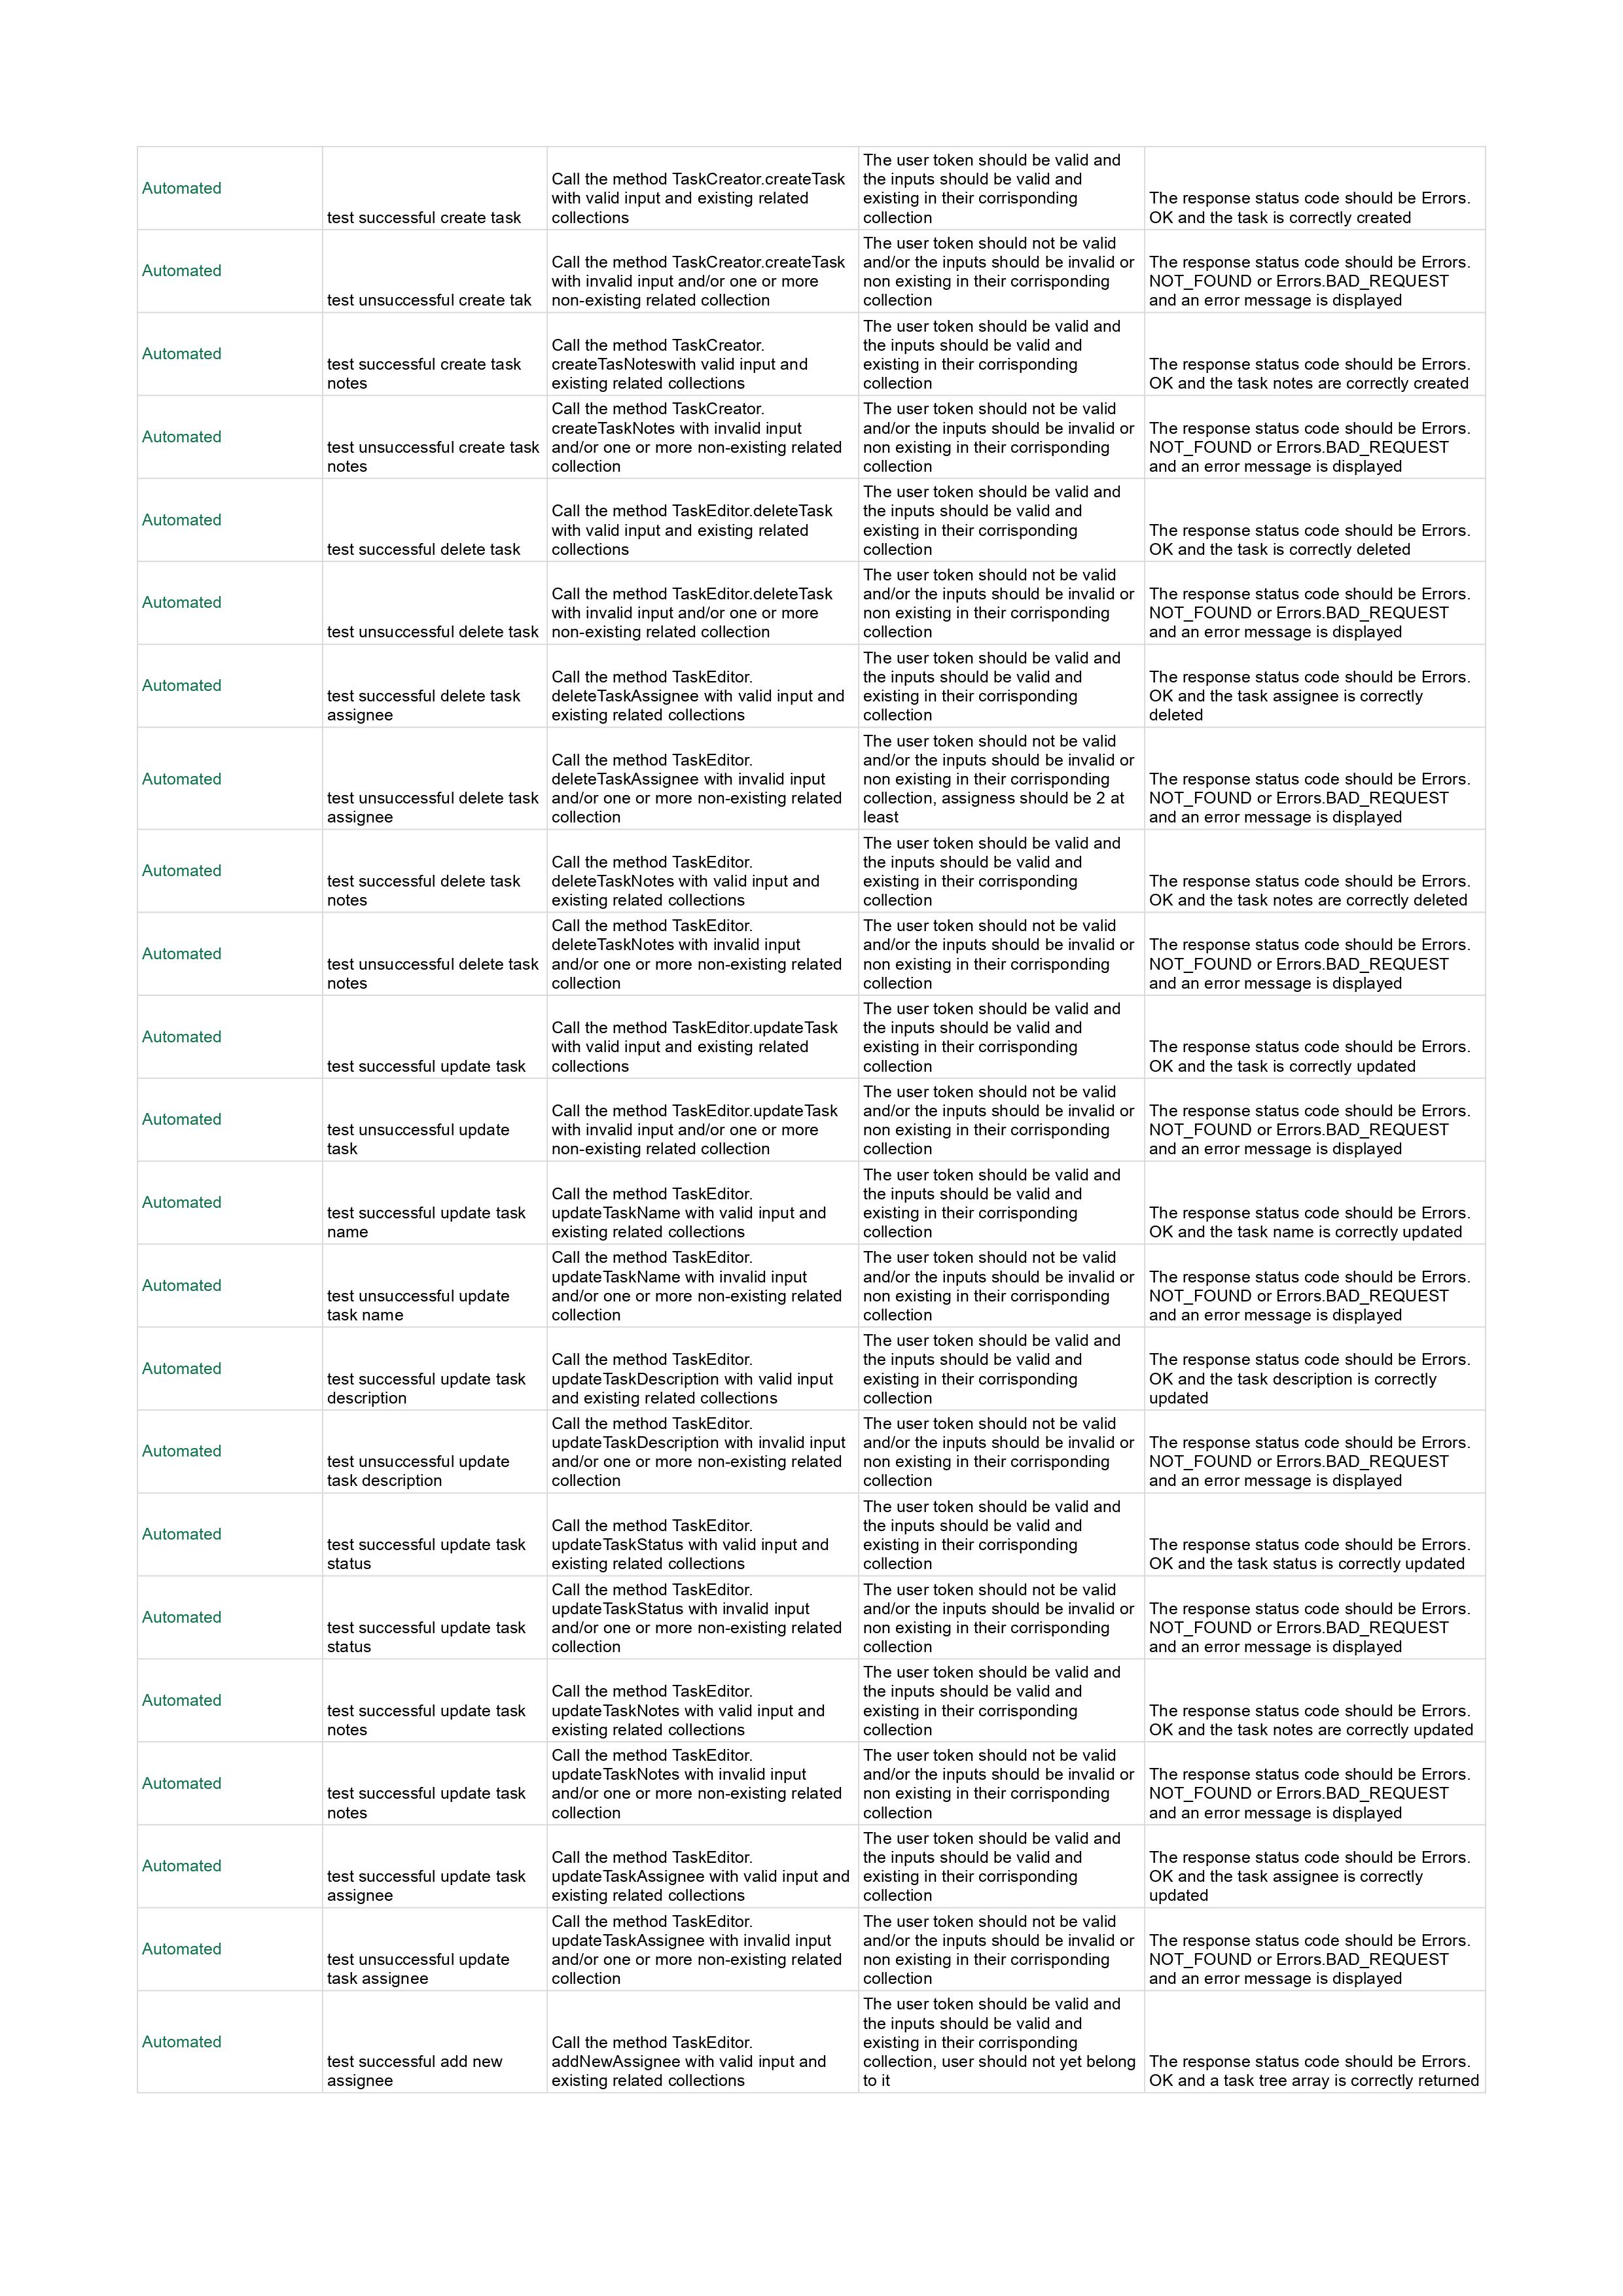
\includegraphics[width=0.95\textwidth]{images/Test_TaskManager-immagini-0.jpg}
\newline
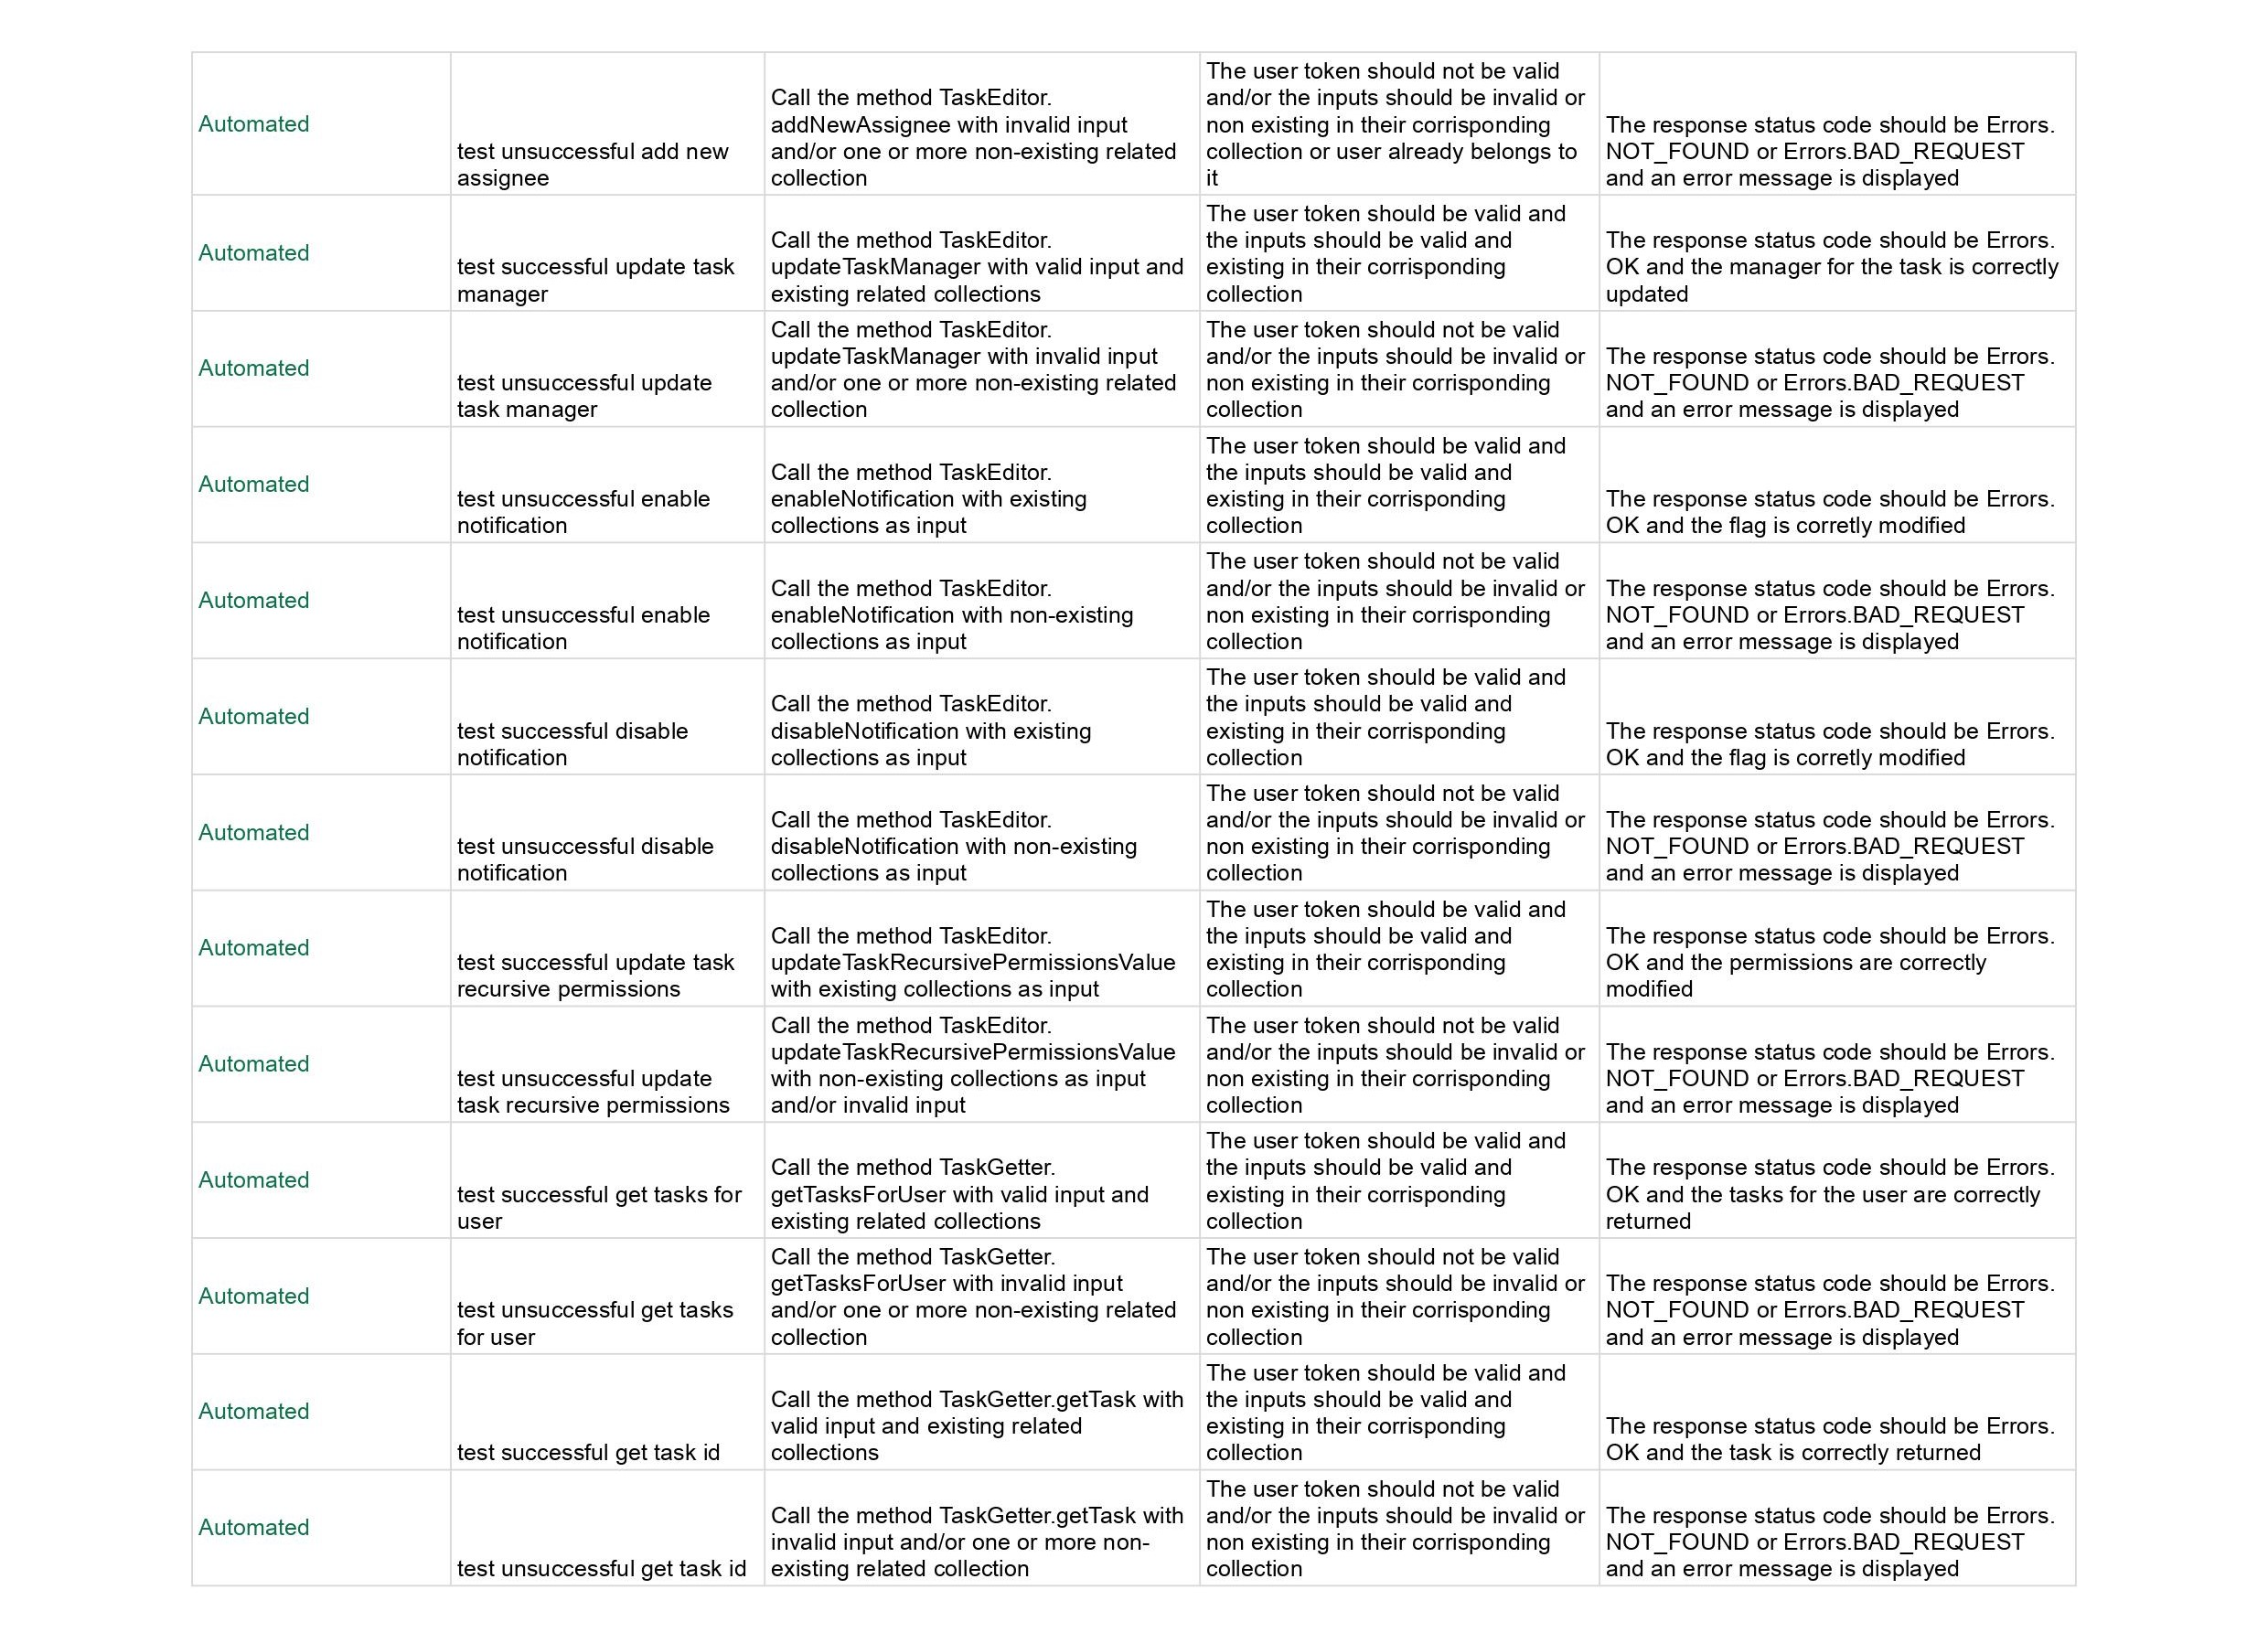
\includegraphics[width=0.95\textwidth]{images/Test_TaskManager-immagini-1.jpg}

\subsection*{Test Home Page}
This section includes manual tests for the home page.
\newline
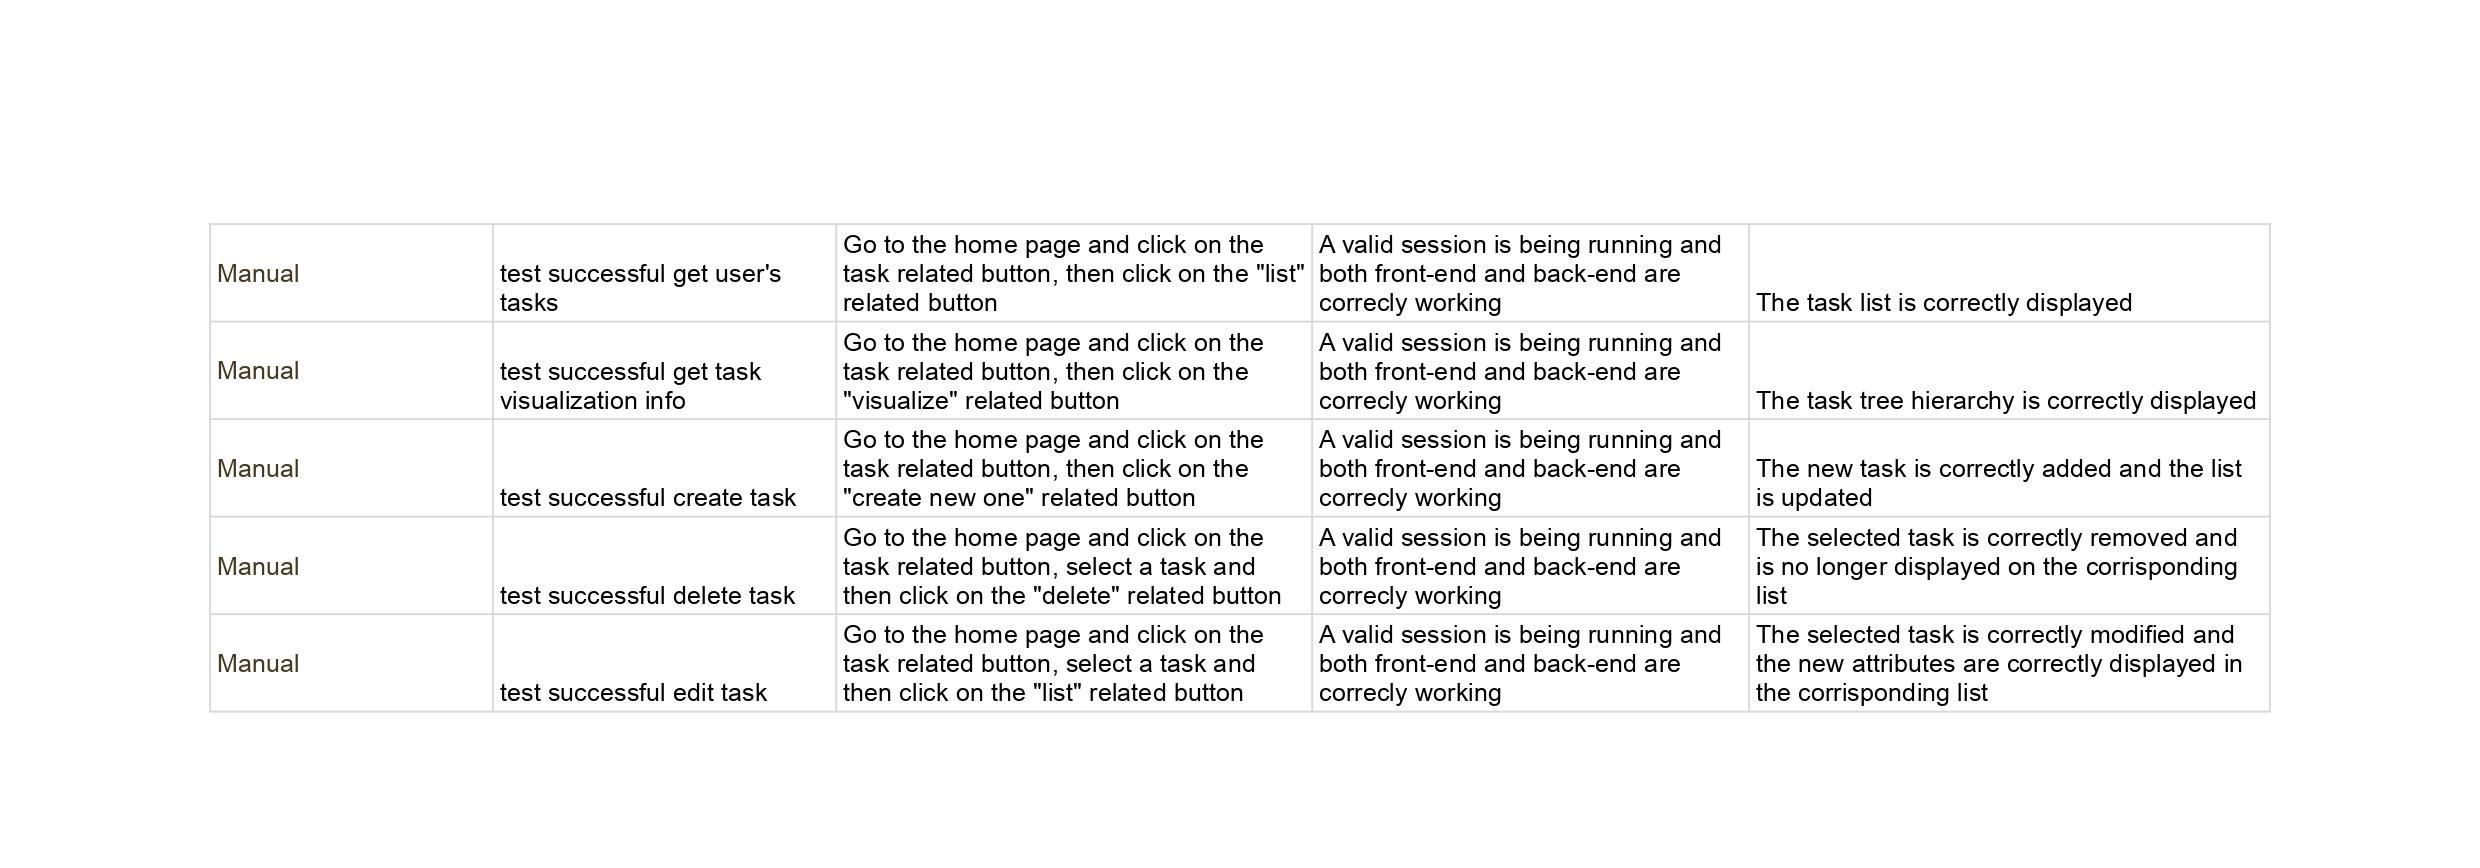
\includegraphics[width=0.95\textwidth]{images/Test_HomePage.jpg}

\subsection*{Test Notification View}
This section includes manual tests for the notification view.
\newline
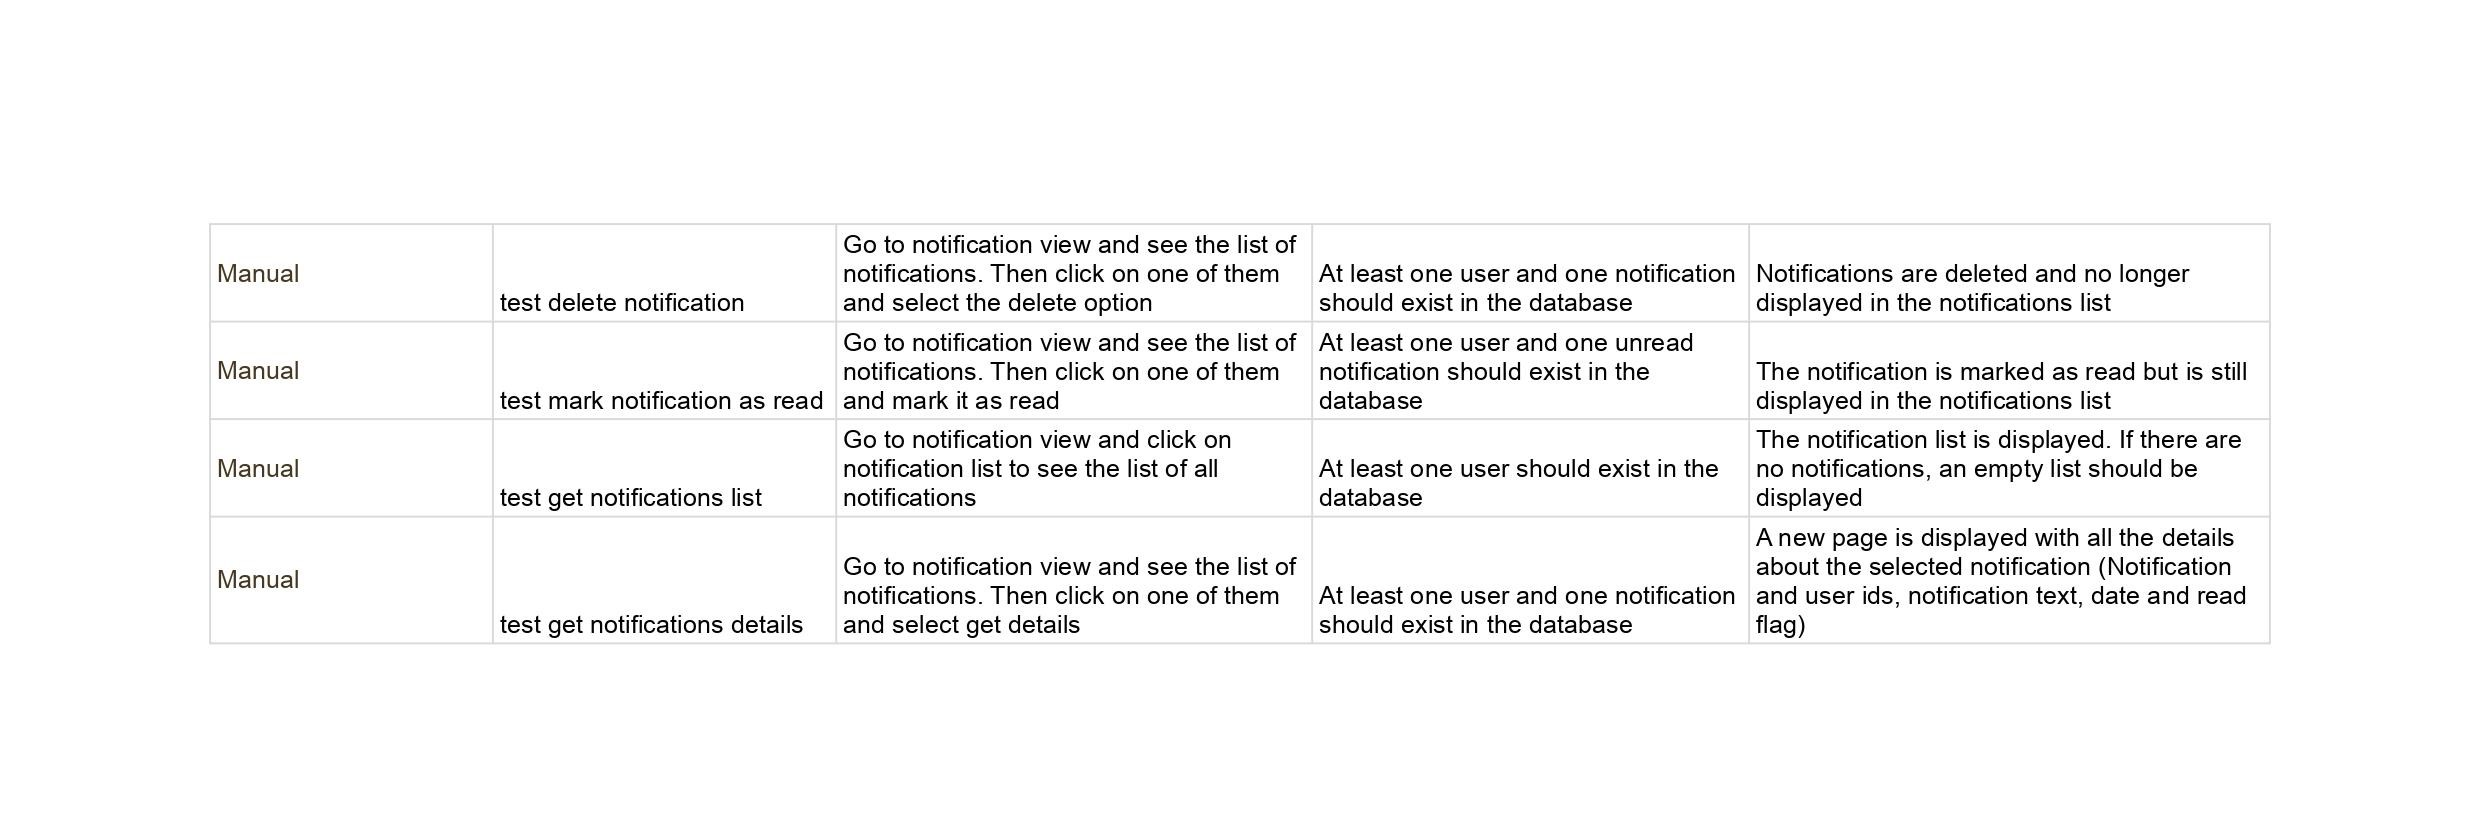
\includegraphics[width=0.95\textwidth]{images/Test_NotificationView.jpg}

\subsection*{Test Sign In and Sign Up Pages}
This section includes manual tests for the sign in and sign up pages.
\newline
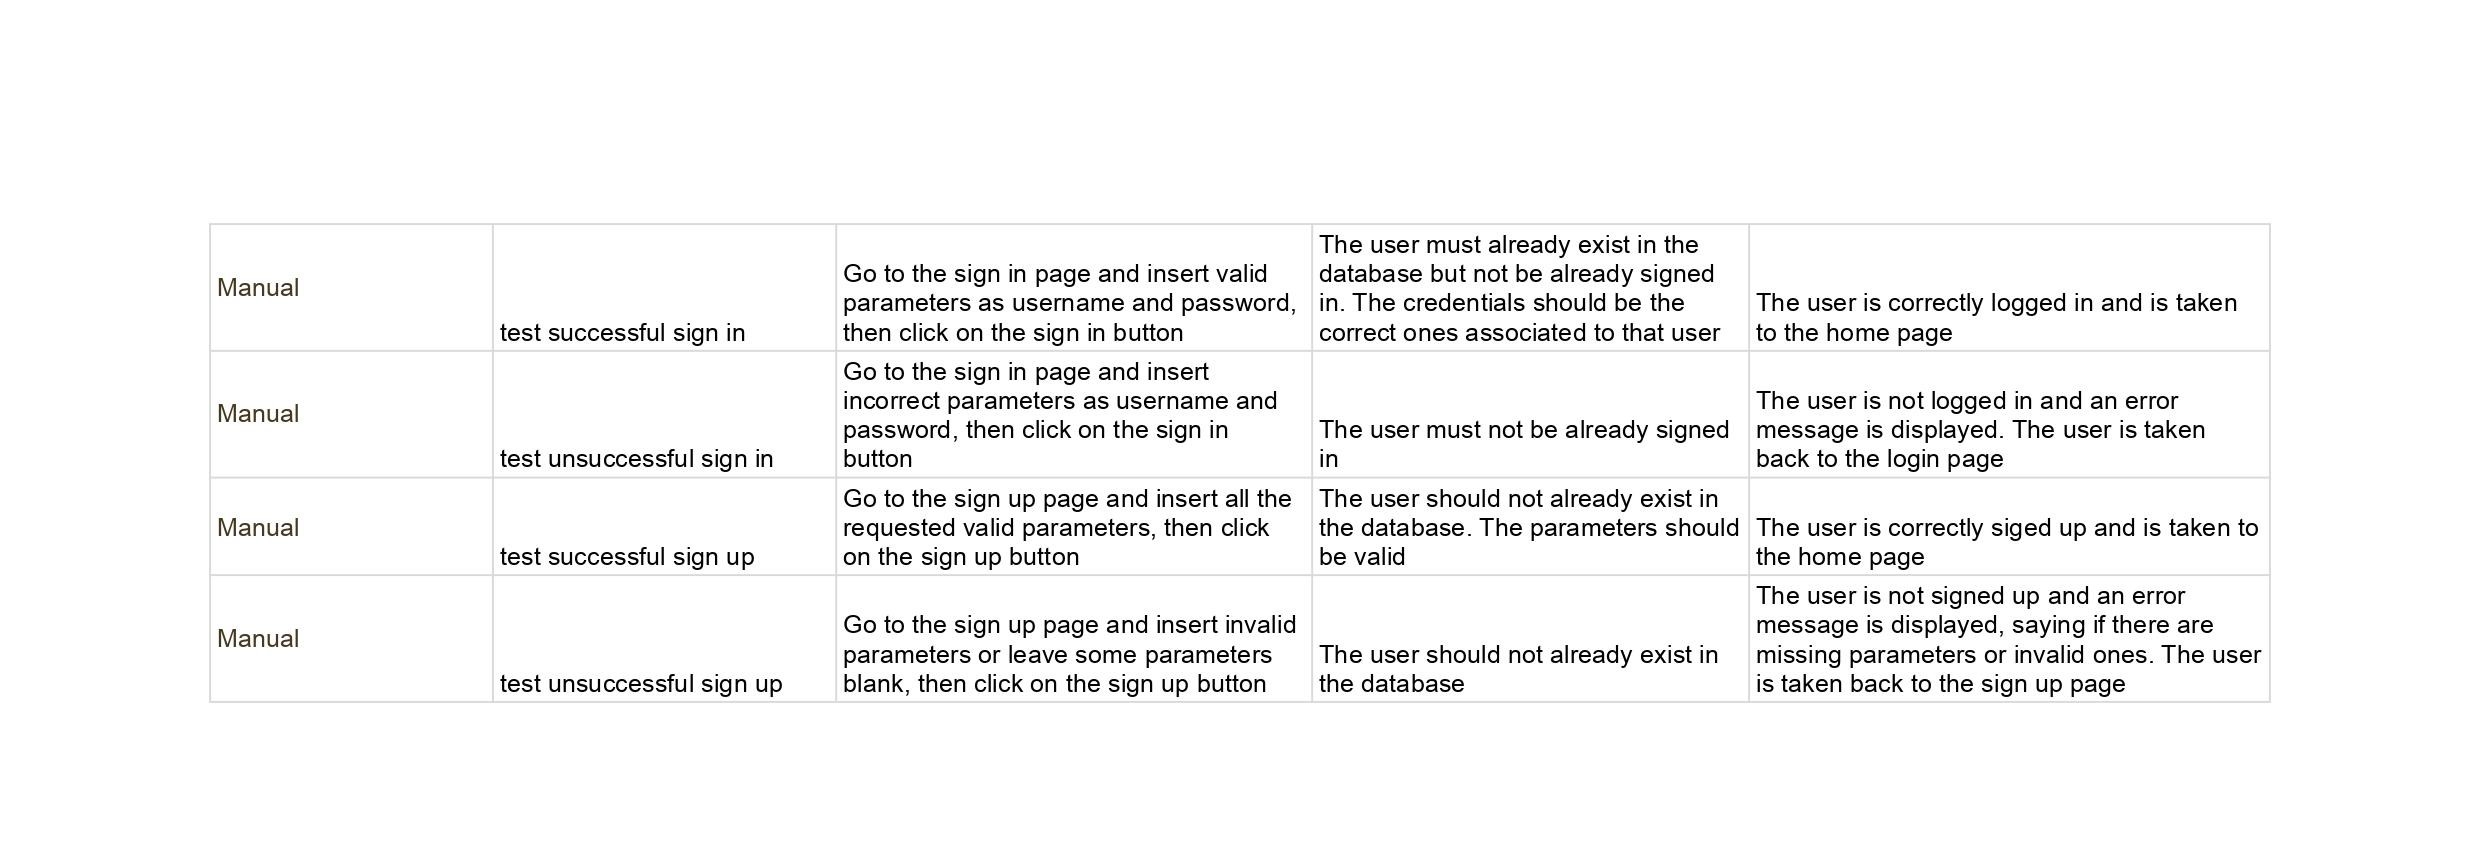
\includegraphics[width=0.95\textwidth]{images/Test_SignInSignUpPage.jpg}

\subsection*{Test Edit Profile Page}
This section includes manual tests for the edit profile page.
\newline
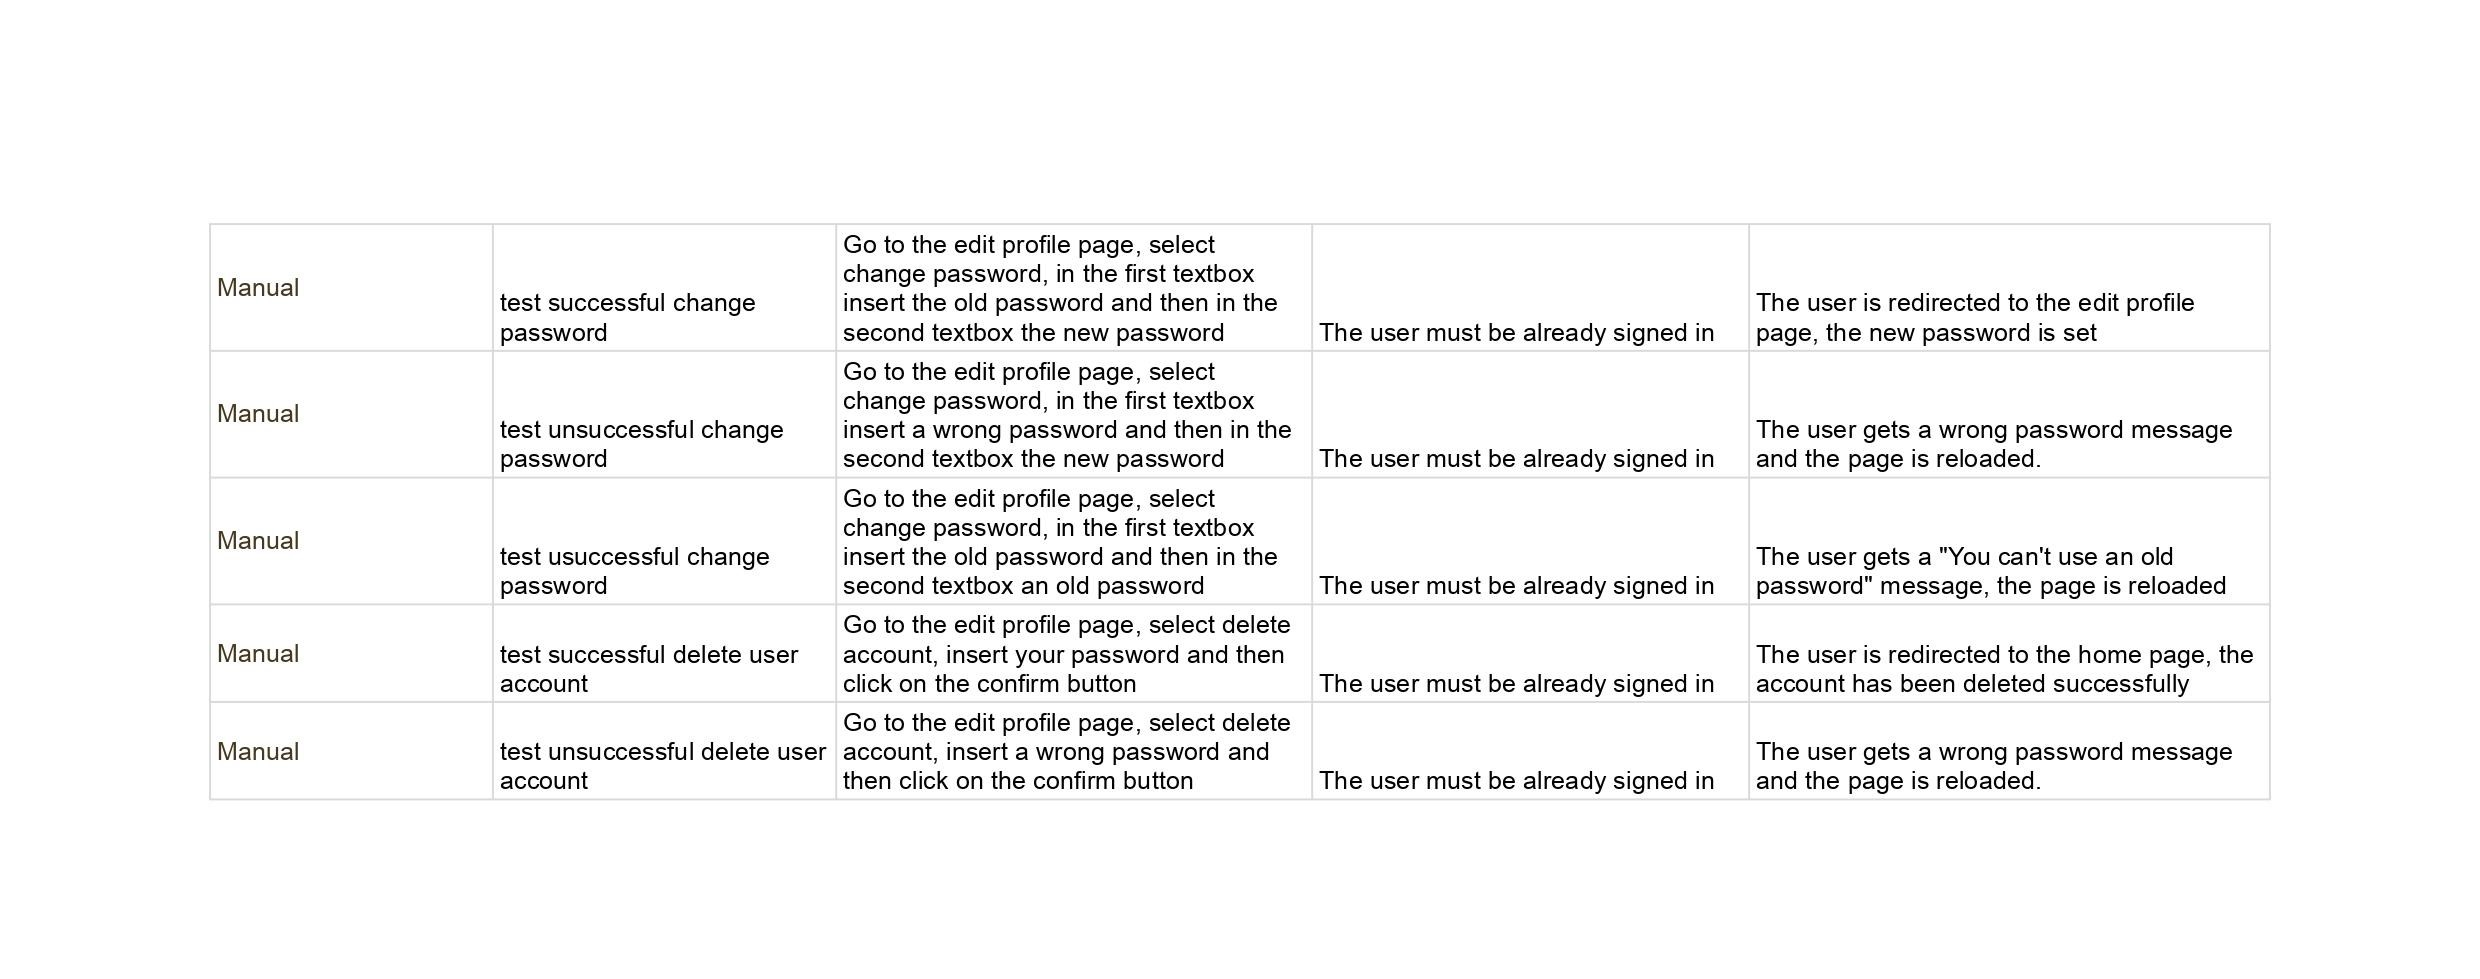
\includegraphics[width=0.95\textwidth]{images/Test_EditProfile.jpg}

\subsection*{Test Organization View Page}
This section includes manual tests for the organization view page.
\newline
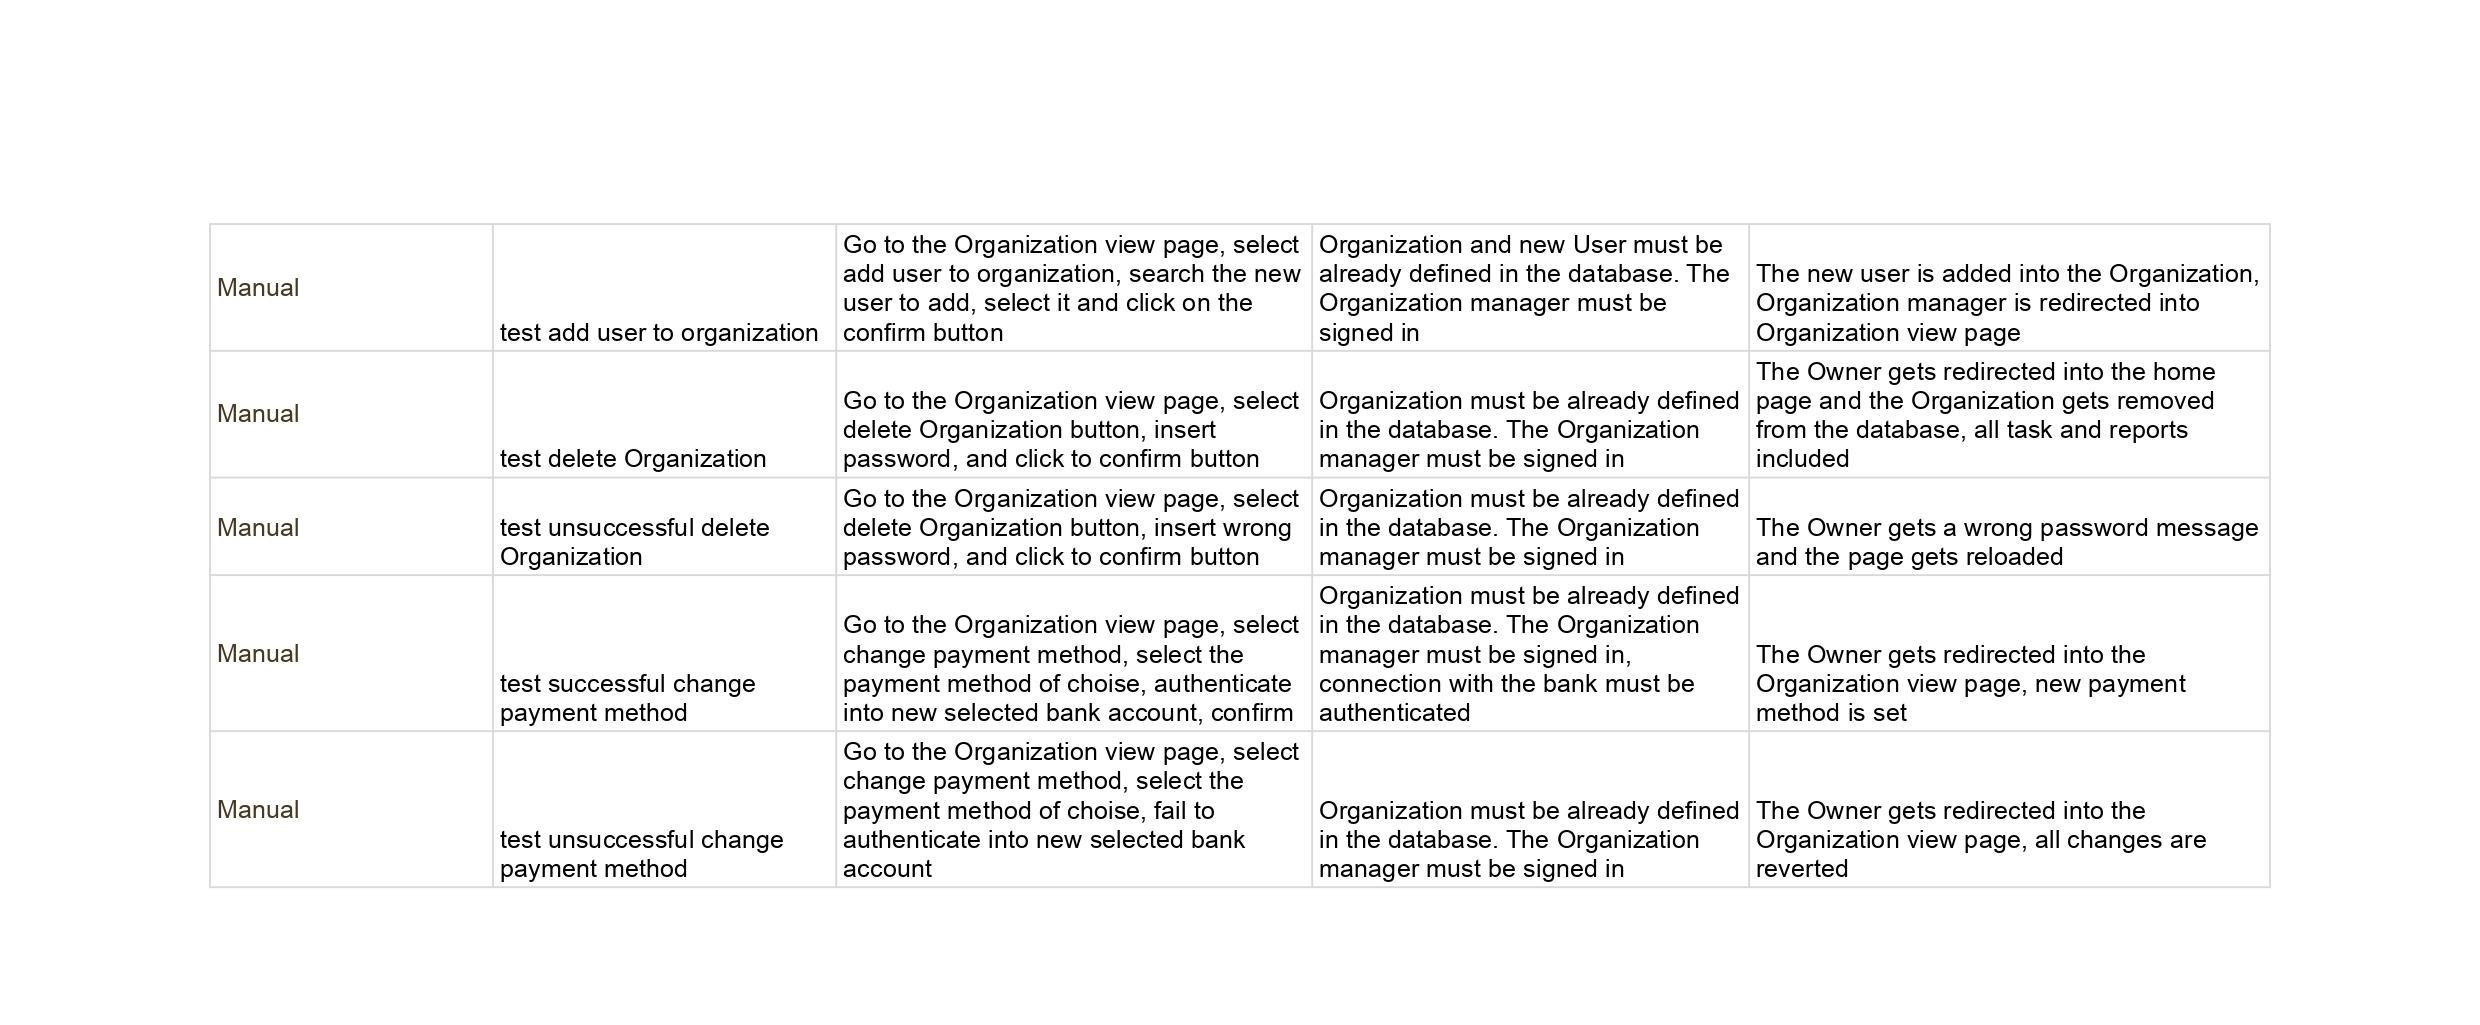
\includegraphics[width=0.95\textwidth]{images/Test_OrganizationView.jpg}

\section{Git Strategy}

Among the several git strategies available and commonly used, we have chosen \textbf{GitHub Flow}. We selected this strategy because it is \textit{one of the simplest} and is particularly suitable for \underline{small teams} like ours. GitHub Flow's straightforward approach, centered around a single branch with short-lived feature branches, allows us to maintain a \textbf{clean and manageable codebase}. This strategy also facilitates \textit{continuous integration and delivery}, making it easier to track progress and integrate changes seamlessly.



\section{Sprint 1}

\subsection{Sprint 1 Backlog}
\includegraphics[width=0.95\textwidth]{images/sprint_backlog.jpg}

\subsection{Sprint 1 Review and Retrospective}

Overall, the sprint was successful, as we managed to complete all the tasks on time.

We experienced some minor slowdowns due to our unfamiliarity with \textit{JavaScript} and \textit{MongoDB}, but we ultimately overcame these challenges. This sprint has been a valuable learning experience, highlighting areas where we can improve our technical skills.

In terms of task estimation, our decision to adopt a \textbf{conservative approach} proved to be beneficial. The higher estimates allowed us to allocate sufficient time to each task, reducing stress and enabling us to handle unforeseen issues effectively.

Team coordination was commendable, though there is room for improvement. The \underline{meticulous division of labor} contributed significantly to our success. Each member had a clear understanding of their responsibilities, which facilitated smoother collaboration and minimized overlapping efforts. However, we need to refine our task distribution further to optimize efficiency.

One notable area for improvement is our handling of \textbf{code integration}. Merging diverging branches proved to be time-consuming and occasionally disrupted our workflow. To address this, we should implement more frequent integration practices and establish clearer guidelines for branch management. This will help us avoid the pitfalls of merging conflicts and enhance our overall productivity.

Looking ahead to the upcoming sprint, we should focus on better organizing the workload across the team. By distributing tasks more evenly and ensuring that everyone is aligned with our coding standards and best practices, we can mitigate potential bottlenecks and maintain a steady progress rate.

Additionally, we should continue to invest time in learning and mastering the technologies we are using. This will not only boost our efficiency but also increase the quality of our product.

In conclusion, while this sprint has been a success, it also highlighted several areas for potential growth. By addressing these issues and building on our strengths, we can look forward to an even more productive standard for out team as a whole.

\subsection{Burndown Chart}
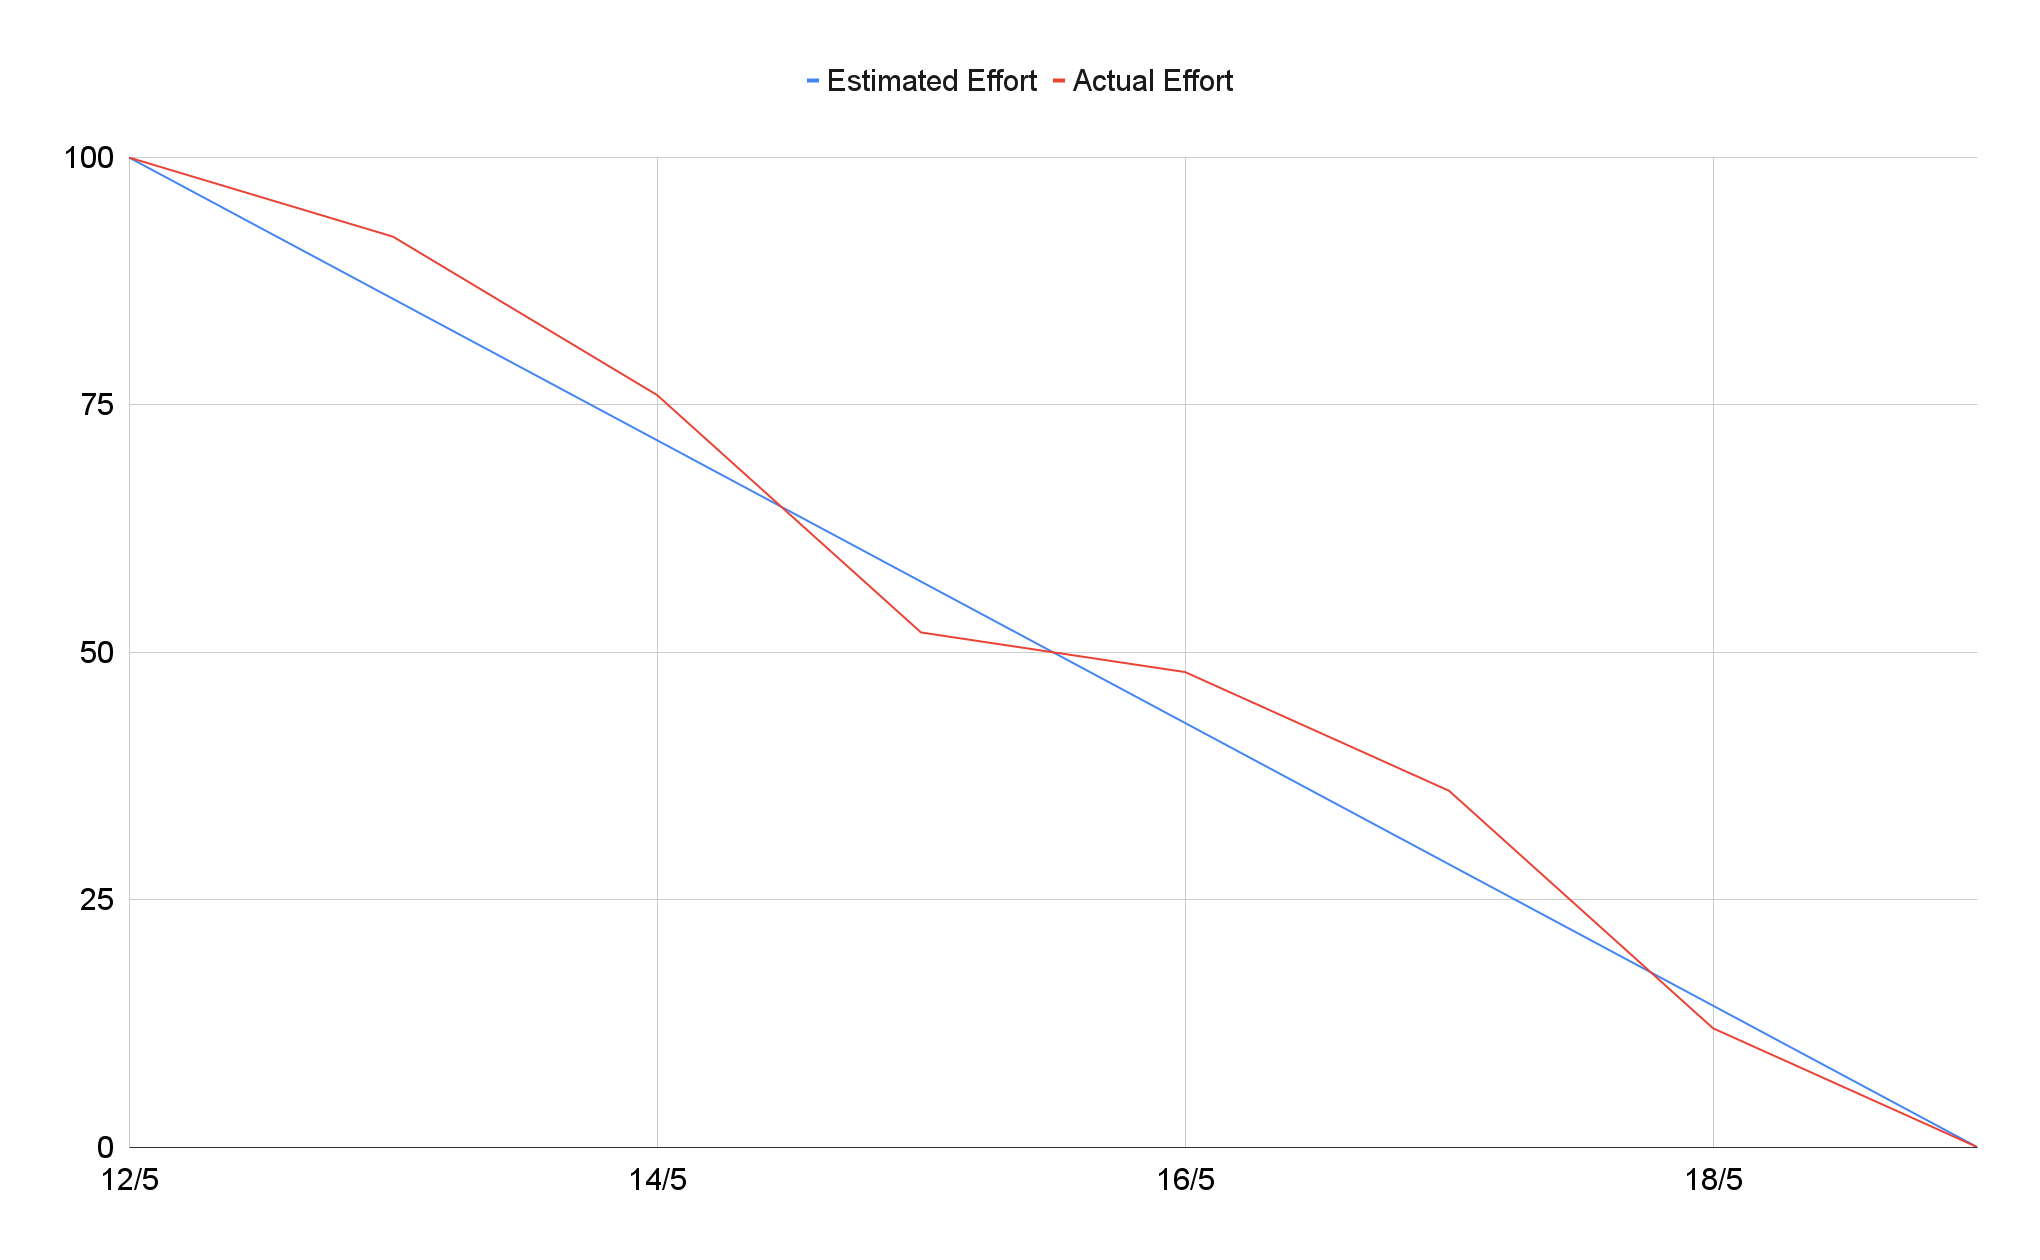
\includegraphics[width=0.95\textwidth]{images/burndown_chart.png}



\end{document}

